% ============================================================================
% SmartTask — University of Dhaka, Institute of Information Technology (IIT)
% Project Report (LaTeX content — paste into your report-class skeleton)
%
% Fill in [INSERT ...] placeholders with your personal details / figures.
% ============================================================================

% ----------------------------------------------------------------------------
% FRONT MATTER (adjust to your skeleton's cover page)
% ----------------------------------------------------------------------------
% \chapter*{Acknowledgement}
% ...
% \chapter*{Declaration}
% ...
% \chapter*{Signature Page}
% ...

% ----------------------------------------------------------------------------
% ABSTRACT
% ----------------------------------------------------------------------------
\begin{abstract}
Task management in team-based software environments is frequently hindered by
disconnected tools, delayed status propagation, and weak accountability. This
project presents \textbf{SmartTask}, a real-time collaborative Kanban-based task
management system designed to streamline planning, execution, and review within a
single web application. The system implements a role-based access control model
with three actor types -- Administrator, Manager, and Member -- and provides
interactive drag-and-drop Kanban boards, sprint and epic management, task
checklists, comments with user mentions, time tracking, reviews with automatic
column transitions, attachment upload, automation rules, audit logging, and an
undo mechanism. The front end is built with Next.js and React, while a standalone
Socket.IO server supplies real-time collaboration, and PostgreSQL serves as the
persistent store through the Prisma ORM. Authentication is secured using JSON Web
Tokens stored exclusively in HTTP-only cookies, with session re-validation on
every request. The system was verified through extensive interactive browser-based
testing across all roles and services, and the resulting application is
production-deployed on Vercel and Render. The report documents the complete
analysis, design, implementation, and testing lifecycle of the system.
\end{abstract}

% ----------------------------------------------------------------------------
% CHAPTER 1 — INTRODUCTION
% ----------------------------------------------------------------------------
\chapter{Introduction}

\section{Project Overview}
SmartTask is a real-time collaborative Kanban-based task management system. The
application is deployed and publicly accessible at
\url{https://smarttaskio.vercel.app}, with the standalone real-time server hosted
separately on Render. The project demonstrates a production-ready web application
built with a modern TypeScript stack, integrating role-based access control,
agile planning, real-time collaboration, and comprehensive auditability into a
single cohesive platform.

\section{Background}
Modern software teams rely on task management tools to organise work, track
progress, and coordinate members. Popular platforms such as Trello, Jira, and
Asana demonstrate that Kanban-style boards offer an intuitive visual model for
workflow control. However, many such tools are either heavy for small teams,
expensive, or force a fixed workflow that does not adapt to an organisation's
specific process. There is a continuing need for a self-contained task management
system that combines real-time collaboration, granular role-based permissions,
and agile planning constructs such as sprints and epics in a single, manageable
application.

\section{Project Motivation}
The motivation behind SmartTask is threefold. First, most existing tools separate
the Kanban board from sprint planning, backlog grooming, and review activities,
forcing users to switch between modules and losing context. Second, real-time
collaboration -- where one user's board update is instantly visible to others --
requires careful engineering of WebSocket infrastructure and authentication that
is frequently omitted in academic projects. Third, accountability in team settings
depends on audit trails and controlled permissions, which demand a well-designed
role model and logging mechanism. SmartTask addresses all three concerns in one
integrated platform.

\section{Objectives}
The primary objectives of this project are:
\begin{itemize}
  \item To design and implement a role-based task management system supporting
        three actor types (Administrator, Manager, and Member).
  \item To provide interactive Kanban boards with drag-and-drop task movement and
        work-in-progress (WIP) limit enforcement.
  \item To support agile planning through sprints, epics, backlogs, and
        sprint-level metrics such as burndown and velocity.
  \item To deliver real-time collaboration using a standalone Socket.IO server.
  \item To secure the application using JWT-based, HTTP-only-cookie authentication
        with session re-validation.
  \item To maintain an audit trail and an undo mechanism for accountability and
        error recovery.
\end{itemize}

\section{Scope}
The scope of the project includes board, column, and task management; comments,
mentions, reactions, checklists, attachments, and time tracking; reviews with
automatic workflow transitions; sprint and epic lifecycle management; automation
rules; notification preferences; system administration; audit logging; and
offline-aware caching through a service worker. The system is delivered as a web
application and is deployed for production use.

\section{Core Modules of the System}
\begin{center}
\begin{tabular}{|l|p{10.5cm}|}
\hline
\textbf{Module} & \textbf{Description} \\
\hline
Authentication & Login, logout, sign-up, password reset, HTTP-only-cookie JWT
sessions with session re-validation, profile and password management. \\
\hline
Role-Based Access Control & Three roles (Administrator, Manager, Member) enforced
by proxy middleware and server-action guards on every route and mutation. \\
\hline
Board Management & Create, edit, delete boards; manage members and tags; board
templates; board analytics. \\
\hline
Column Management & Create, rename, reorder, delete columns; per-column WIP
limits. \\
\hline
Task Management & Create, edit, delete, move tasks; priority, assignee, due
dates, issue fields, labels. \\
\hline
Kanban Board & Drag-and-drop task movement with optimistic updates, WIP
enforcement, and live multi-user updates. \\
\hline
Comments and Mentions & Comment threads, user mentions, emoji reactions,
5-minute edit window for non-privileged users. \\
\hline
Checklists & Create checklists and items, toggle completion, edit and delete. \\
\hline
Attachments & Server-side file upload, database-backed blob storage, secure
download and preview. \\
\hline
Time Tracking & Log, edit, and delete time entries per task. \\
\hline
Reviews & Submit for review, approve/request changes/reject, automatic column
transitions. \\
\hline
Sprint Management & Sprint CRUD, status lifecycle, capacity, review notes,
retro notes and action items. \\
\hline
Sprint Planning & Two-panel planning board, sprint board, calendar, burndown,
velocity, and metrics. \\
\hline
Epic Management & Epic CRUD, status state machine, task assignment. \\
\hline
Automation & Configurable rules triggered by task events, system-wide or
board-scoped. \\
\hline
Notifications & Real-time notification delivery, per-event preferences, read
and unread state. \\
\hline
Audit Logging & Immutable log of every significant action with actor, target,
and metadata; CSV export. \\
\hline
Undo & 30-second undo window that reverses the most recent action. \\
\hline
Offline Support & Service-worker caching and offline-aware behaviour. \\
\hline
\end{tabular}
\end{center}

\section{Thesis Organisation}
The remainder of this report is organised as follows. Chapter~\ref{ch:lit} reviews
related work. Chapter~\ref{ch:analysis} presents the system analysis and
requirements. Chapter~\ref{ch:design} describes the system design and UML
diagrams. Chapter~\ref{ch:implementation} details the implementation.
Chapter~\ref{ch:testing} reports testing and results. Chapter~\ref{ch:conclusion}
concludes the work and discusses future directions.

% ----------------------------------------------------------------------------
% CHAPTER 2 — LITERATURE REVIEW
% ----------------------------------------------------------------------------
\chapter{Literature Review}
\label{ch:lit}

\section{Kanban Methodology}
The Kanban method originated from the Toyota Production System and was adapted to
knowledge work by David J.~Anderson. Its core principles are to visualise work,
limit work in progress, and manage flow. SmartTask implements these principles
through visual columns, WIP limits that are enforced for member-level users, and
column-level statistics exposed through analytics dialogs.

\section{Existing Task Management Systems}
\subsection{Trello}
Trello popularised the card-and-board metaphor. It offers flexible boards, labels,
checklists, and automation through Butler. Its primary limitation is the lack of
sprint and backlog constructs, which made it less suitable for formal agile
delivery teams.
\subsection{Jira Software}
Jira provides deep agile support, including scrum boards, sprints, epics,
burndown charts, and granular permissions. Jira is powerful but heavyweight, and
its workflow configuration can be intimidating for small teams. SmartTask adopts
Jira's sprint and epic concepts while keeping the interface lightweight.
\subsection{Asana}
Asana focuses on project tracking, task assignments, and timelines. Its
permissions model is comparatively flat, and real-time board collaboration is less
emphasised than in dedicated Kanban tools.

\section{Comparison and Gap Analysis}
The reviewed tools share several gaps that SmartTask addresses: (i)~integrated
sprint planning and review within the same board experience; (ii)~a clear
three-role permission model that prevents members from altering board structure;
(iii)~real-time presence and live board updates; and (iv)~an audit trail with an
undo mechanism for accountability. These gaps informed the functional
requirements presented in the next chapter.

% ----------------------------------------------------------------------------
% CHAPTER 3 — SYSTEM ANALYSIS AND REQUIREMENTS
% ----------------------------------------------------------------------------
\chapter{System Analysis and Requirements}
\label{ch:analysis}

\section{Problem Statement}
Teams require a single platform that supports visual task tracking, structured
planning, controlled permissions, and real-time awareness. Existing solutions are
either too simple to support sprints or too complex for everyday use. SmartTask
aims to provide the right balance while remaining fully self-contained and
deployable.

\section{User Roles and Permissions}
The system defines three actor types:
\begin{itemize}
  \item \textbf{Administrator (ADMIN):} full access across all boards; user
        management (create, edit, delete, change role); system-wide audit logs and
        reports; global and board automation rules; board and column management on
        any board.
  \item \textbf{Manager (MANAGER):} manages the boards they own or belong to;
        creates and deletes boards and columns; sets WIP limits; adds or removes
        members; creates sprints and epics; approves reviews; may override WIP
        limits.
  \item \textbf{Member (MEMBER):} works on assigned boards; creates and edits
        tasks, comments, checklists, and time entries; moves tasks subject to WIP
        limits; submits reviews; cannot create boards or columns, cannot manage
        members, and cannot change roles.
\end{itemize}

\section{Functional Requirements}
\subsection{Authentication and Account Management}
\begin{itemize}
  \item FR-01: The system shall allow login, logout, sign-up, and password reset.
  \item FR-02: Sessions shall be stored in HTTP-only cookies as JSON Web Tokens.
  \item FR-03: Users shall be able to update their profile, avatar, and password.
  \item FR-04: Notification preferences shall be configurable per user.
\end{itemize}
\subsection{Board and Column Management}
\begin{itemize}
  \item FR-05: Administrators and Managers shall create, edit, and delete boards.
  \item FR-06: Board members shall be managed by administrators and managers.
  \item FR-07: Columns shall be created, renamed, reordered, and deleted.
  \item FR-08: WIP limits shall be configurable per column and enforced for members.
\end{itemize}
\subsection{Task Management}
\begin{itemize}
  \item FR-09: Members shall create, edit, and delete tasks on assigned boards.
  \item FR-10: Tasks shall support title, description, priority, assignee, dates,
        labels, and issue fields.
  \item FR-11: Tasks shall be moved between columns by drag-and-drop.
  \item FR-12: Checklists, attachments, time entries, and issue links shall be
        supported per task.
  \item FR-13: Comments with user mentions and emoji reactions shall be supported.
\end{itemize}
\subsection{Reviews}
\begin{itemize}
  \item FR-14: Users shall submit tasks for review by selecting a reviewer.
  \item FR-15: Self-review shall be blocked.
  \item FR-16: Approving a review shall move the task to the done column;
        requesting changes shall move it to the in-progress column; rejection shall
        move it to the first column.
\end{itemize}
\subsection{Sprints and Epics}
\begin{itemize}
  \item FR-17: Managers shall create, edit, delete, and change the status of
        sprints following a defined state machine.
  \item FR-18: Tasks shall be assignable to and removable from sprints.
  \item FR-19: Completing a sprint shall return incomplete tasks to the backlog.
  \item FR-20: Epics shall support create, edit, delete, and status transitions.
\end{itemize}
\subsection{Automation and Notifications}
\begin{itemize}
  \item FR-21: Administrators and Managers shall define automation rules triggered
        by task events.
  \item FR-22: The system shall generate and deliver notifications and respect
        per-user preferences.
\end{itemize}
\subsection{Administration and Auditing}
\begin{itemize}
  \item FR-23: Administrators shall manage system users and roles.
  \item FR-24: The system shall log every significant action in an audit trail.
  \item FR-25: Users shall be able to undo their most recent action within a
        30-second window.
\end{itemize}

\section{Non-Functional Requirements}
The system shall be secure, using HTTP-only cookies, bcrypt password hashing,
role-based access checks at both the middleware and server-action layers, and
server-side validation of all inputs. It shall be reliable, with atomic database
transactions guarding critical operations such as sprint status changes and WIP
enforcement. It shall be performant, rendering pages through server components and
lazy-loading heavy client libraries. It shall be real-time, delivering board and
notification updates over WebSocket connections. It shall be maintainable, using
TypeScript across the codebase, a central validation layer, and consistent server
action patterns. Finally, it shall be accessible and responsive, adapting to
mobile viewports without horizontal overflow.

\section{System Feasibility}
\subsection{Technical Feasibility}
The required technologies -- Next.js, React, TypeScript, Prisma, PostgreSQL, and
Socket.IO -- are mature, well-documented, and free to use. The architecture
separates the persistent application (Next.js) from the real-time layer
(Socket.IO), both of which were deployed successfully, confirming technical
feasibility.
\subsection{Economic Feasibility}
All components are open-source or free-tier hosted services. The application runs
on Vercel and Render free tiers, and the database on a free Supabase tier,
resulting in near-zero operating cost.
\subsection{Operational Feasibility}
The role-based interface is intuitive, with clear separation of capabilities.
Deployment is automated through continuous integration, and the audit trail aids
operational accountability.

% ----------------------------------------------------------------------------
% CHAPTER 4 — SYSTEM DESIGN AND UML DIAGRAMS
% ----------------------------------------------------------------------------
\chapter{System Design and UML Diagrams}
\label{ch:design}

\section{Architecture Overview}
SmartTask follows a client--server architecture with two server components. The
Next.js application serves the user interface and implements business logic
through server actions and API routes. A standalone Socket.IO server maintains
persistent WebSocket connections for real-time collaboration and executes
background jobs for due-date reminders and audit-log cleanup. Both servers access
a shared PostgreSQL database through independent Prisma clients.

\begin{figure}[h]
  \centering
  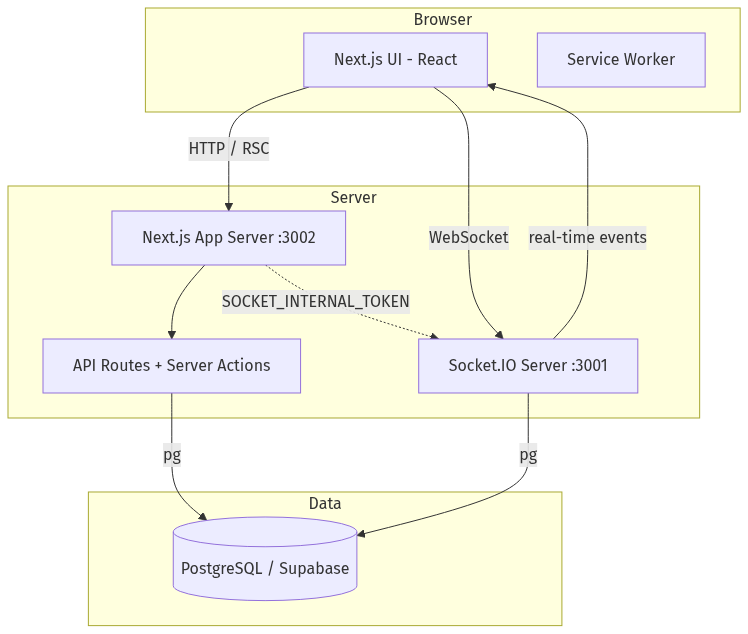
\includegraphics[width=0.9\textwidth]{figures/system-architecture}
  \caption{High-level system architecture showing the browser, the Next.js
  application server, the standalone Socket.IO server, and the shared PostgreSQL
  database.}
\end{figure}
\noindent As shown in Figure~\ref{...}, the browser communicates with the Next.js
server over HTTP for page rendering and server actions, and establishes a
WebSocket connection to the Socket.IO server for real-time events. The Socket.IO
server authenticates incoming connections using the same session token issued by
the application server, and the two servers coordinate through an internal token
that grants the application server the privilege to notify any user.

\subsection{Role-Based System Architecture}
The system is architected around three roles, each with a clearly bounded set of
responsibilities that is enforced at two layers: the proxy middleware, which
guards every route request, and the server-action layer, which re-validates
permissions before every mutation.
\begin{itemize}
  \item \textbf{Administrator Architecture:} The administrator operates the
        highest tier, with access to user management, system-wide audit logs,
        global and board automation rules, and every board across the
        organisation. All administrative pages reside under the
        \texttt{/admin} route segment, which is protected by an admin-only guard.
  \item \textbf{Manager Architecture:} Managers operate at the board tier. They
        own or belong to boards and can create boards, columns, sprints, and
        epics; manage members; set WIP limits; and approve reviews. Manager
        routes under \texttt{/manager} are accessible to managers and
        administrators only.
  \item \textbf{Member Architecture:} Members operate at the task tier. They
        create and edit tasks, comments, checklists, and time entries, and move
        tasks subject to WIP limits on boards they are assigned to. Member routes
        under \texttt{/member} are open to every authenticated user, but
        structure-level actions are blocked at the action layer.
\end{itemize}
This layered model ensures that hiding a button in the interface is not the only
defence: direct URL access and raw action invocation are both rejected for
unauthorised roles, as verified during testing.

\section{Use Case Diagram}
\begin{figure}[h]
  \centering
  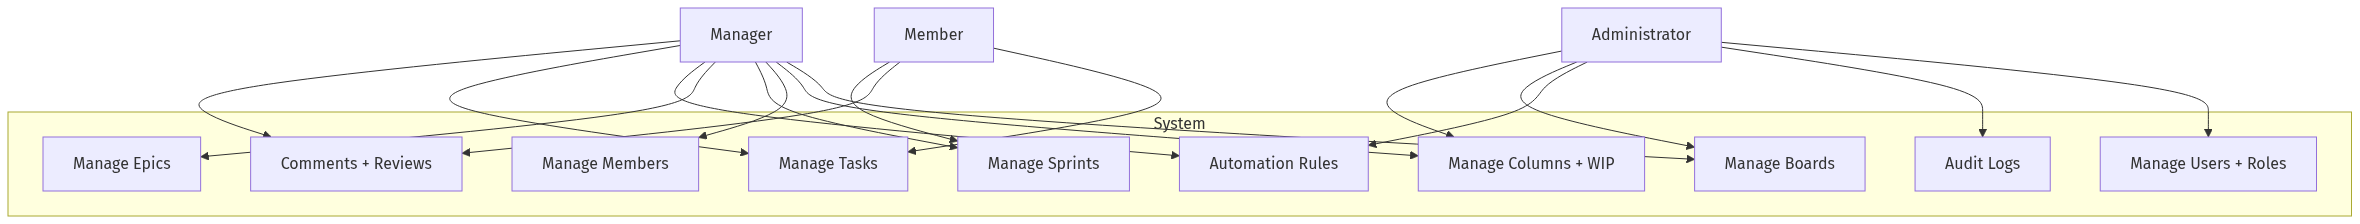
\includegraphics[width=0.95\textwidth]{figures/use-case-diagram}
  \caption{Use case diagram showing the primary actors (Administrator, Manager,
  Member) and their interactions with boards, tasks, sprints, epics, reviews,
  notifications, and administrative functions.}
\end{figure}
\noindent The Administrator is the only actor able to manage system users, roles,
and global automation rules. The Manager inherits member capabilities and, within
boards they own, may manage boards, columns, members, sprints, and epics. The
Member is restricted to task-level collaboration on assigned boards and cannot
alter board structure.

\section{Class / ER Diagram}
\begin{figure}[h]
  \centering
  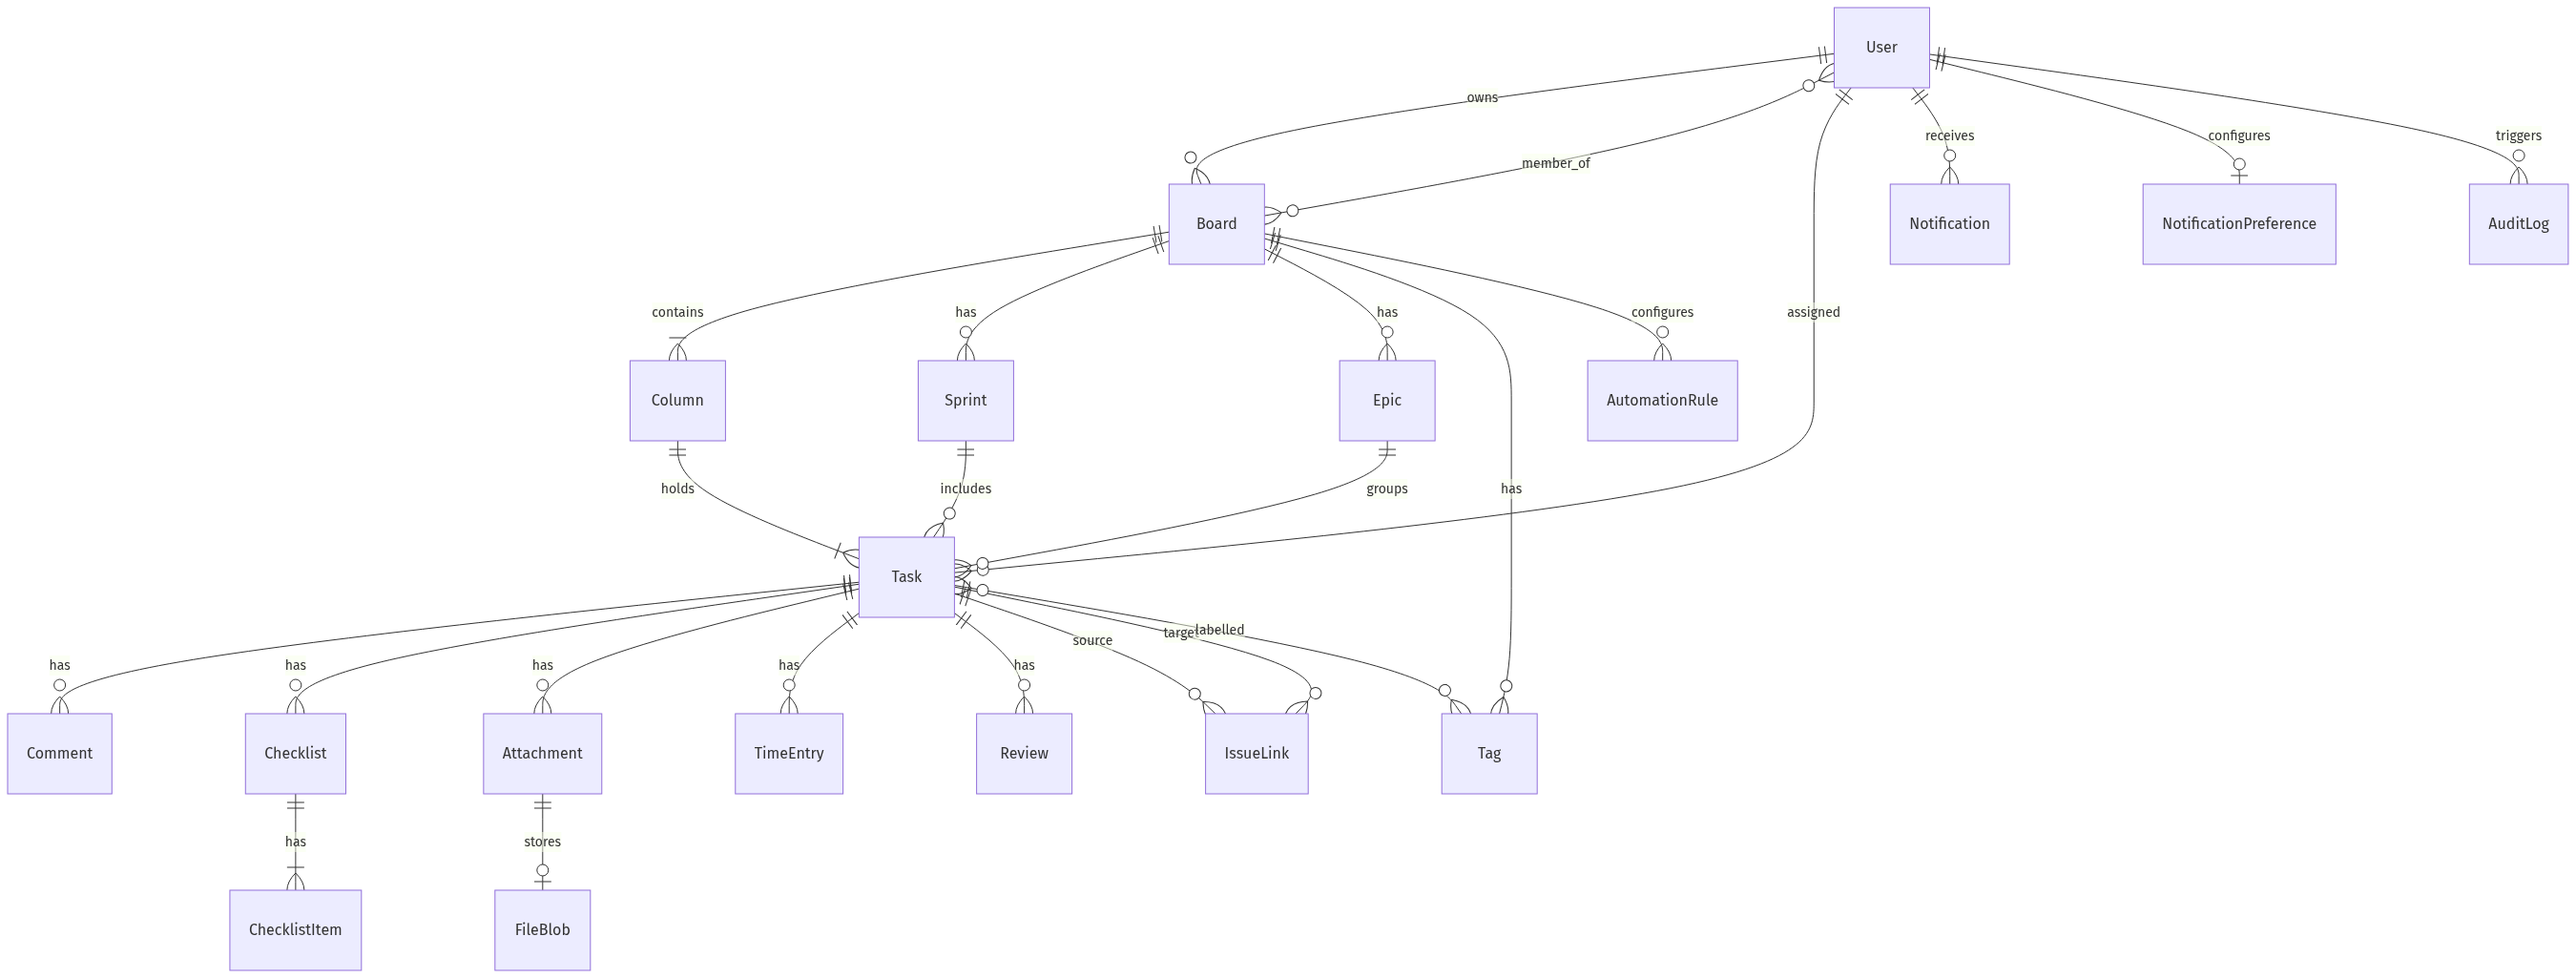
\includegraphics[width=0.95\textwidth]{figures/er-diagram}
  \caption{Entity--relationship diagram of the core database schema.}
\end{figure}
\noindent The schema centres on the \texttt{User} entity, which relates to boards
through ownership and membership relations. Each \texttt{Board} contains multiple
\texttt{Column}s, and each \texttt{Column} contains \texttt{Task}s. Tasks relate to
comments, reactions, attachments (with an associated file blob), checklists,
checklist items, time entries, reviews, tags, and issue links. Sprints and epics
associate with boards and tasks. Audit, notification, and automation tables
complete the schema. Twenty-one database models were implemented in total.

\section{Sequence Diagram -- Task Movement with WIP Enforcement}
\begin{figure}[h]
  \centering
  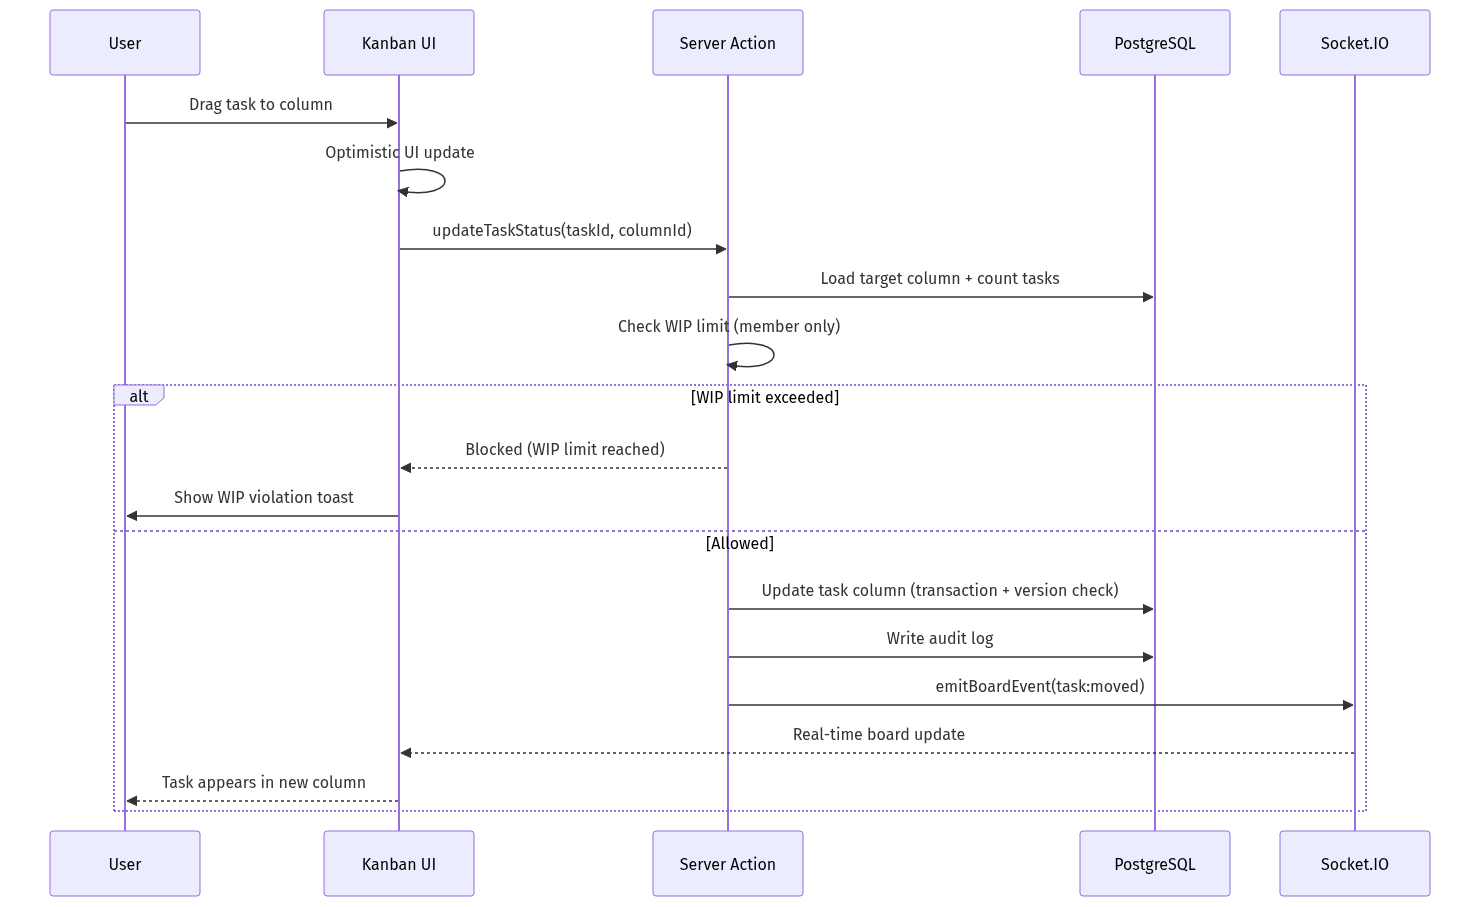
\includegraphics[width=0.95\textwidth]{figures/sequence-task-move}
  \caption{Sequence diagram for moving a task between columns, including the WIP
  limit check performed inside a database transaction.}
\end{figure}
\noindent When a user drags a task to another column, the client emits an
optimistic update and invokes the \texttt{updateTaskStatus} server action. The
action loads the target column, counts the tasks in it, and, for member-level
users, verifies that the WIP limit is not exceeded. The update is committed
atomically, a version-conflict check is performed, an audit entry is written, and
a real-time event is broadcast so that all viewers receive the change.

\section{Activity Diagram -- Sprint Lifecycle}
\begin{figure}[h]
  \centering
  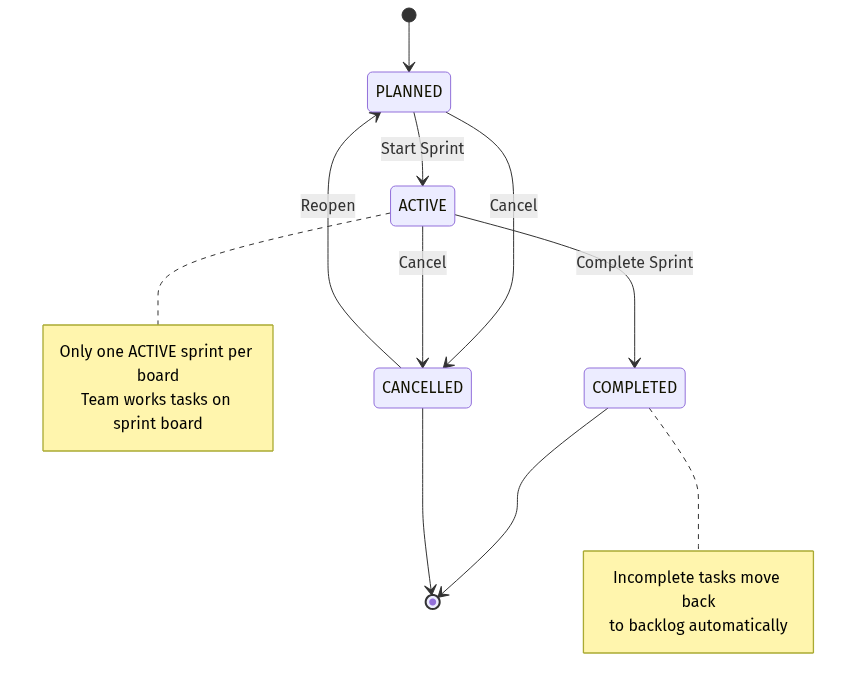
\includegraphics[width=0.9\textwidth]{figures/activity-sprint-lifecycle}
  \caption{Activity diagram of the sprint state machine.}
\end{figure}
\noindent Sprints transition from PLANNED to ACTIVE, then to COMPLETED or
CANCELLED. Only one ACTIVE sprint may exist per board, enforced atomically. When a
sprint is completed, all tasks not in the done column are automatically returned
to the backlog.

% ----------------------------------------------------------------------------
% CHAPTER 5 — IMPLEMENTATION
% ----------------------------------------------------------------------------
\chapter{Implementation}
\label{ch:implementation}

\section{Tools and Technology}
\begin{itemize}
  \item \textbf{Frontend:} Next.js 16 (App Router), React 19, TypeScript,
        Tailwind CSS 4, shadcn/ui components.
  \item \textbf{Backend:} Next.js server actions, API route handlers.
  \item \textbf{Real-time:} Socket.IO (standalone server), socket.io-client.
  \item \textbf{Database:} PostgreSQL with Prisma ORM 7 and the pg driver adapter.
  \item \textbf{Authentication:} jose (JWT), bcryptjs, HTTP-only cookies.
  \item \textbf{State and forms:} Zustand, React Hook Form, Zod 4 validation.
  \item \textbf{Charts and interactions:} Recharts, @dnd-kit, date-fns, Sonner.
  \item \textbf{Deployment:} Vercel (application), Render (Socket.IO server).
\end{itemize}

\section{Project View}
The following screenshots illustrate the principal interfaces of the application,
organised by role and core module. Each figure corresponds to a real screen of the
deployed application. [INSERT FIGURE]

\subsection{Authentication and Account Modules}
\begin{figure}[h]
  \centering
  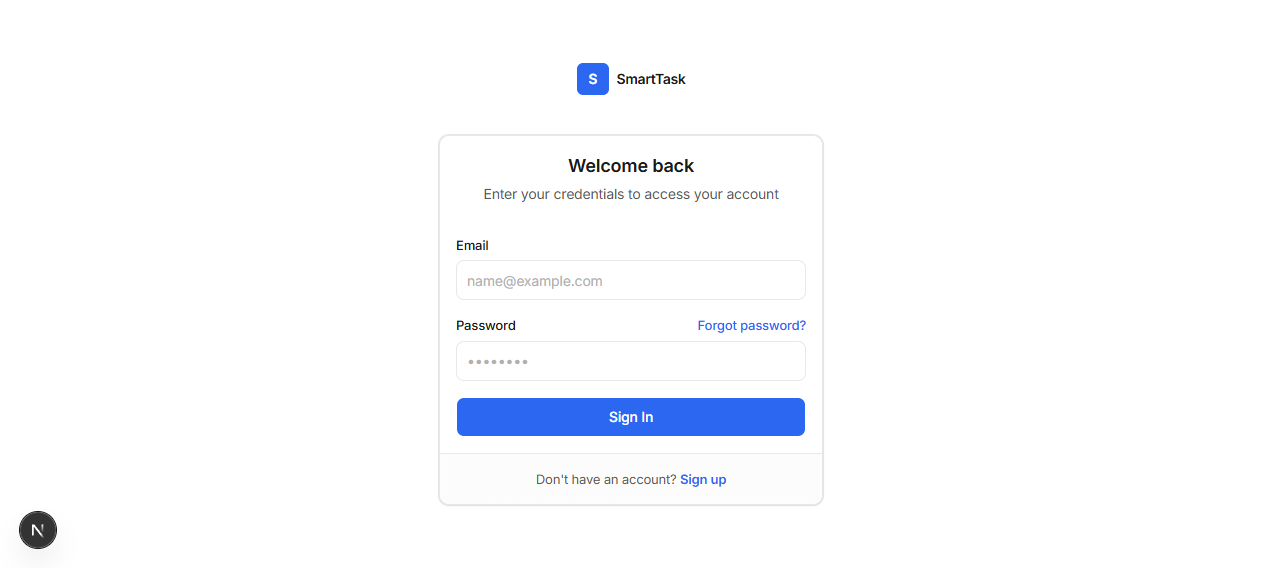
\includegraphics[width=0.9\textwidth]{figures/screenshot-login}
  \caption{Login screen. Authentication is handled by the application server,
  which sets an HTTP-only session cookie.}
\end{figure}

\begin{figure}[h]
  \centering
  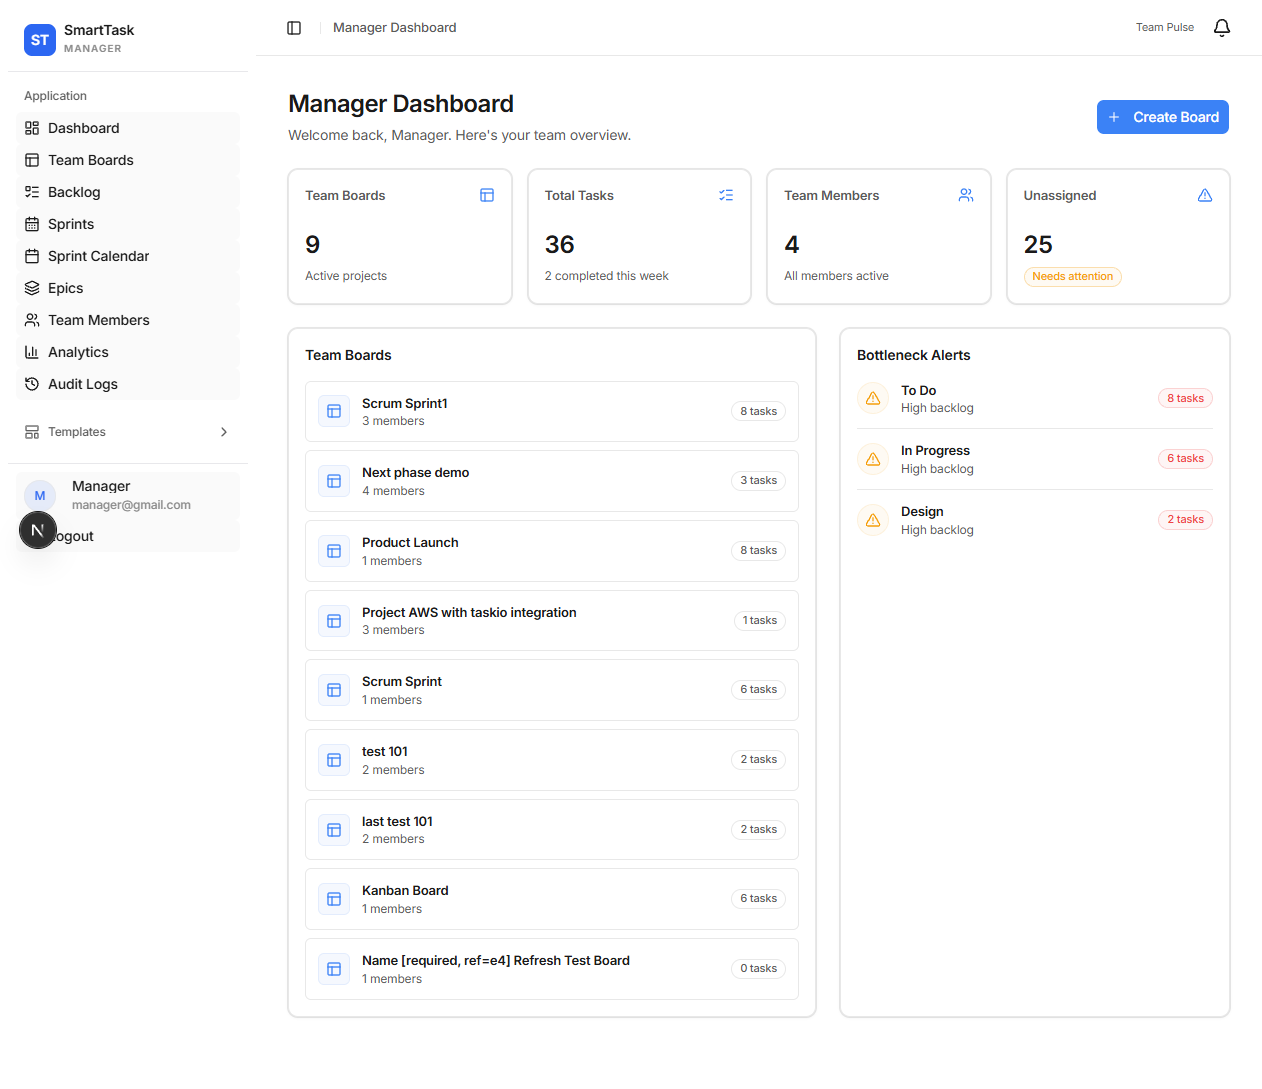
\includegraphics[width=0.9\textwidth]{figures/screenshot-signup}
  \caption{Sign-up screen. New users are created as members and receive a
  welcome board automatically.}
\end{figure}

\begin{figure}[h]
  \centering
  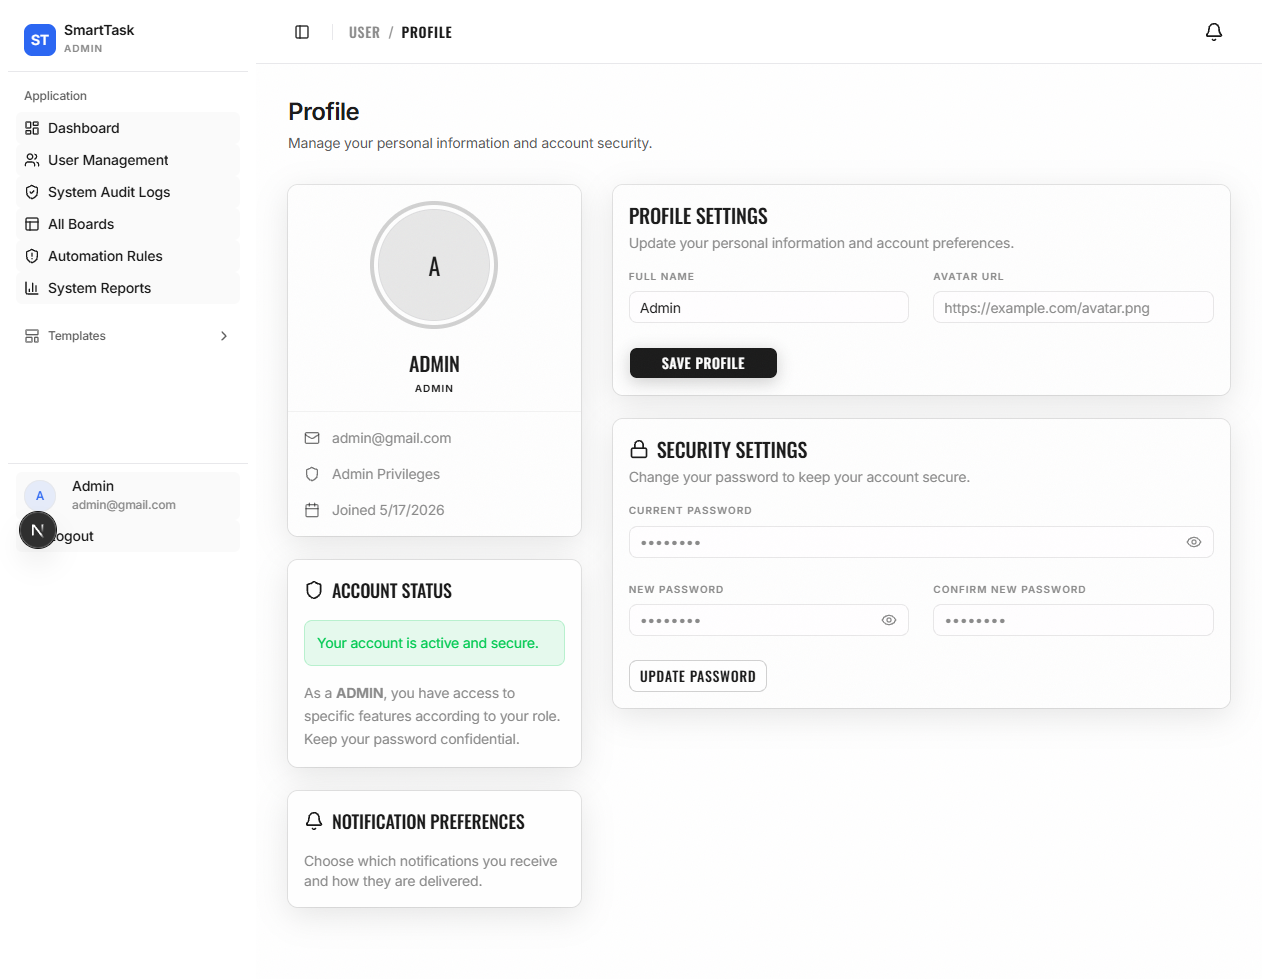
\includegraphics[width=0.9\textwidth]{figures/screenshot-profile}
  \caption{Profile page for updating name, avatar, and password.}
\end{figure}

\begin{figure}[h]
  \centering
  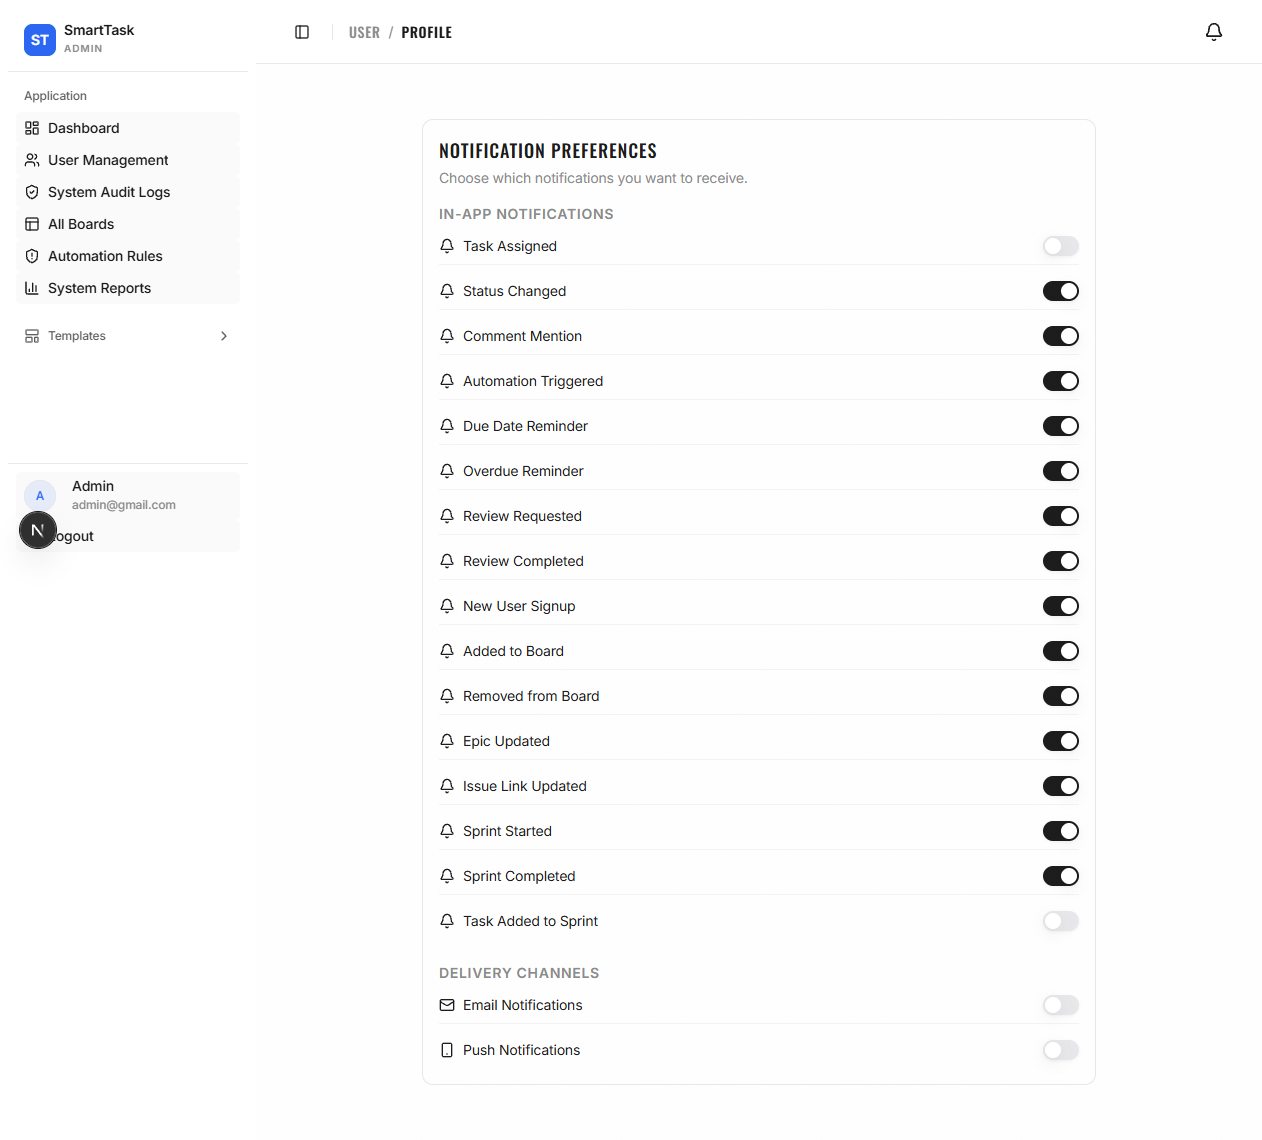
\includegraphics[width=0.9\textwidth]{figures/screenshot-notification-preferences}
  \caption{Notification preferences page with per-event toggles and delivery
  channels.}
\end{figure}

\subsection{Board and Task Management Modules}
\begin{figure}[h]
  \centering
  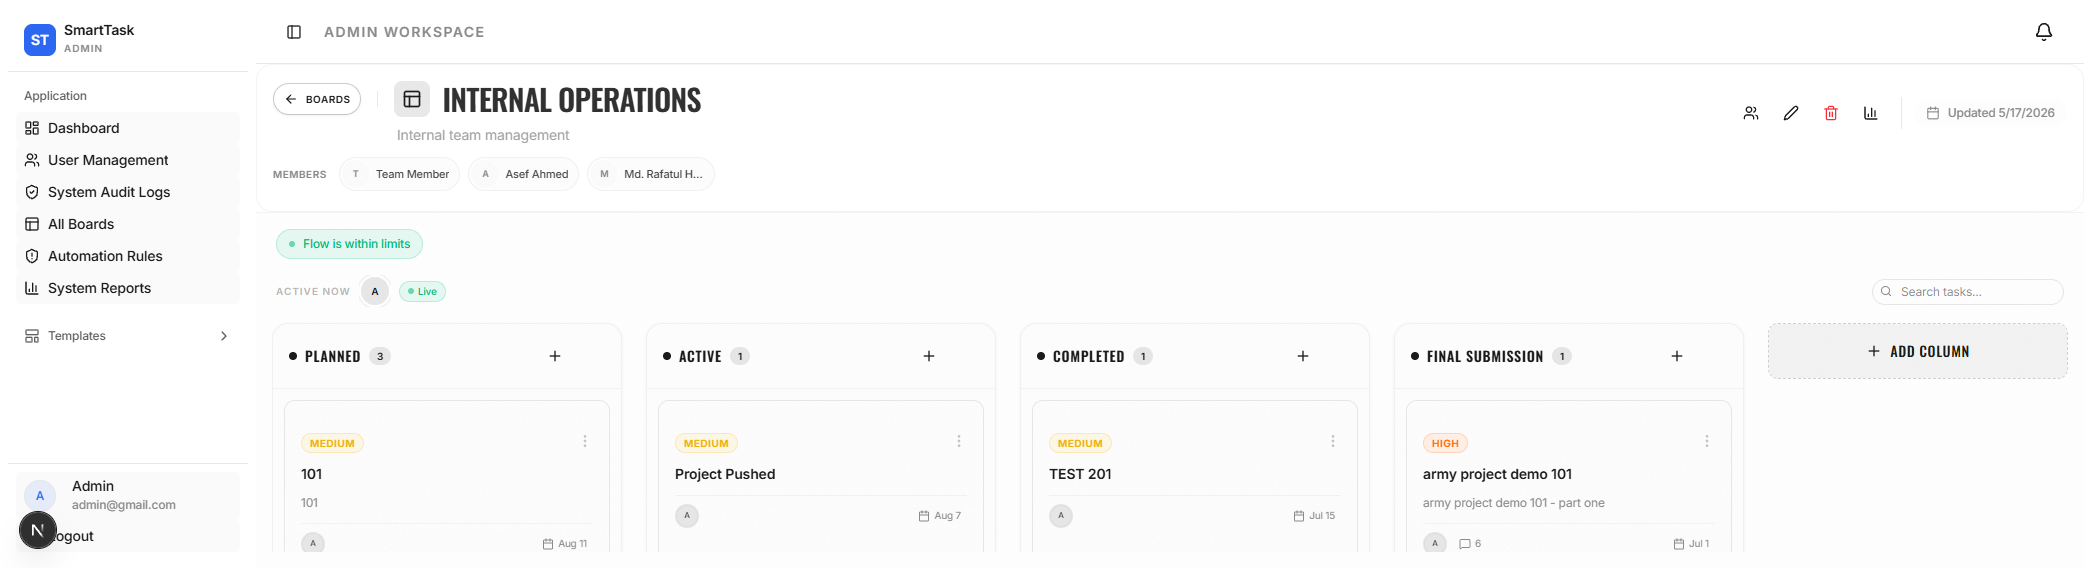
\includegraphics[width=0.9\textwidth]{figures/screenshot-kanban}
  \caption{Kanban board view showing columns, task cards, and column-level
  actions.}
\end{figure}

\begin{figure}[h]
  \centering
  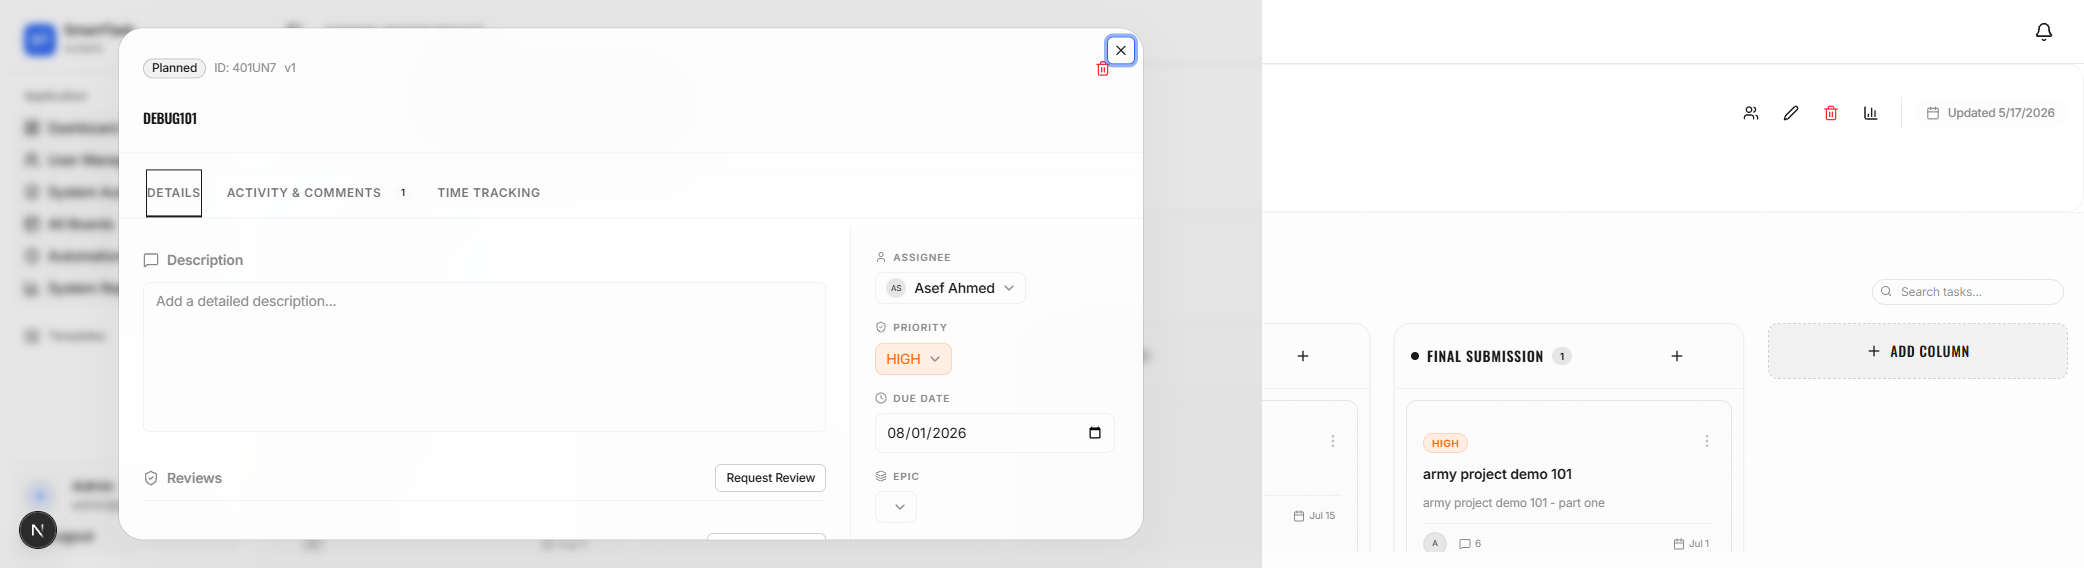
\includegraphics[width=0.9\textwidth]{figures/screenshot-task-details}
  \caption{Task details dialog exposing tabs for details, activity and comments,
  and time tracking, together with review, checklist, attachment, and issue-link
  controls.}
\end{figure}

\begin{figure}[h]
  \centering
  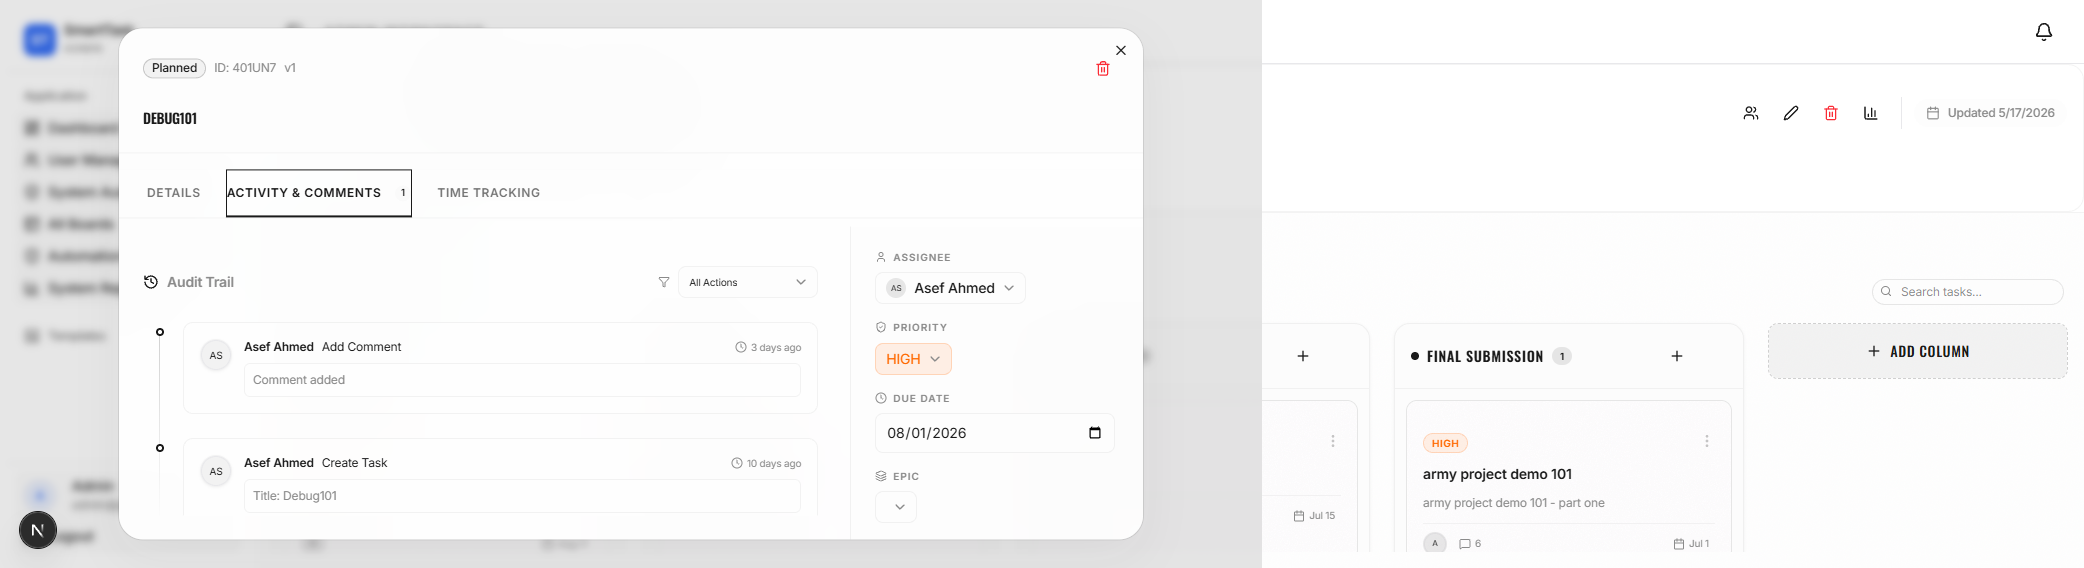
\includegraphics[width=0.9\textwidth]{figures/screenshot-task-comments}
  \caption{Activity and comments tab showing a comment thread with mention
  support.}
\end{figure}

\begin{figure}[h]
  \centering
  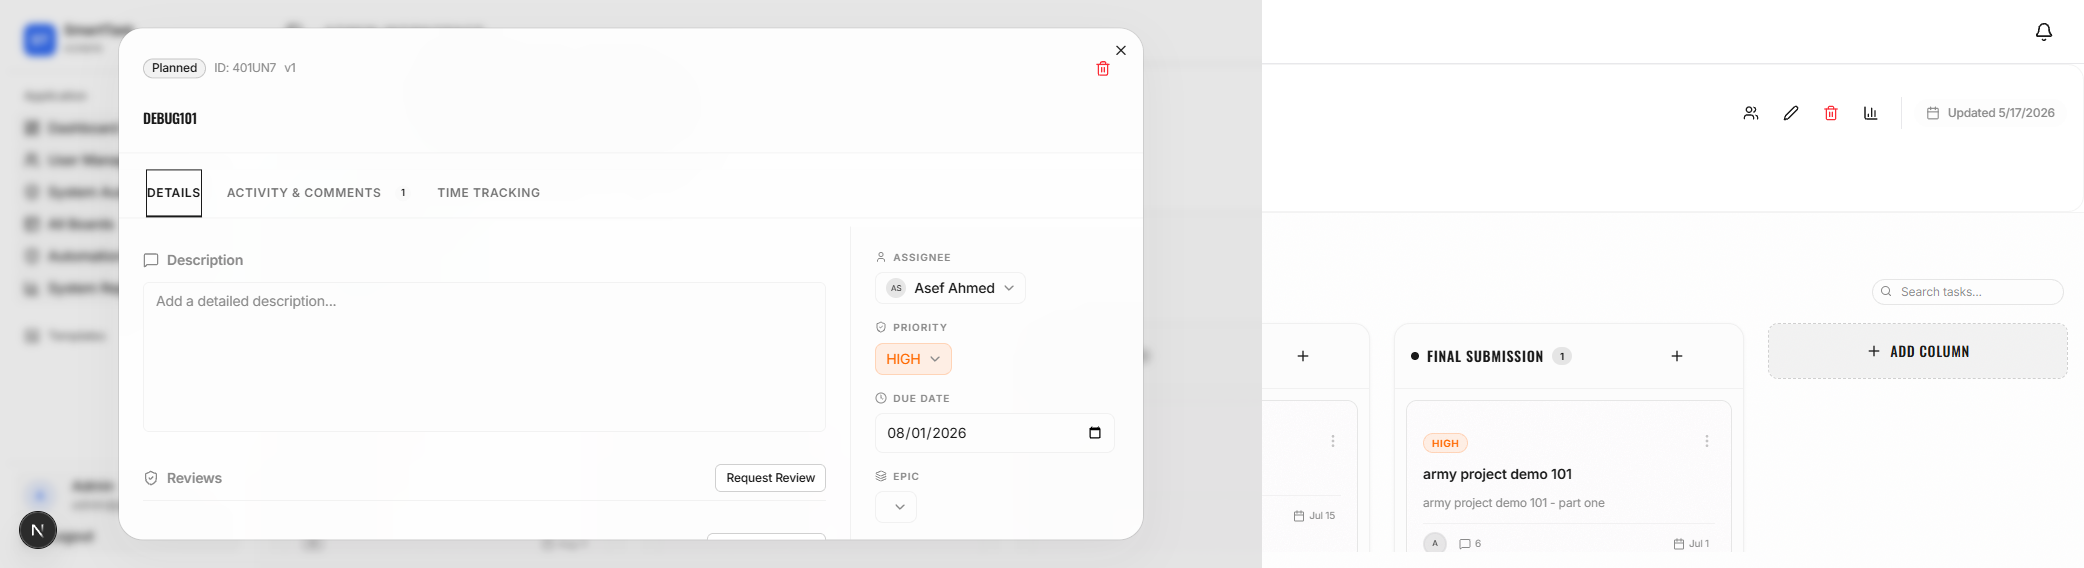
\includegraphics[width=0.9\textwidth]{figures/screenshot-task-review}
  \caption{Review panel with Approve, Request Changes, and Reject actions that
  move the task through the workflow automatically.}
\end{figure}

\begin{figure}[h]
  \centering
  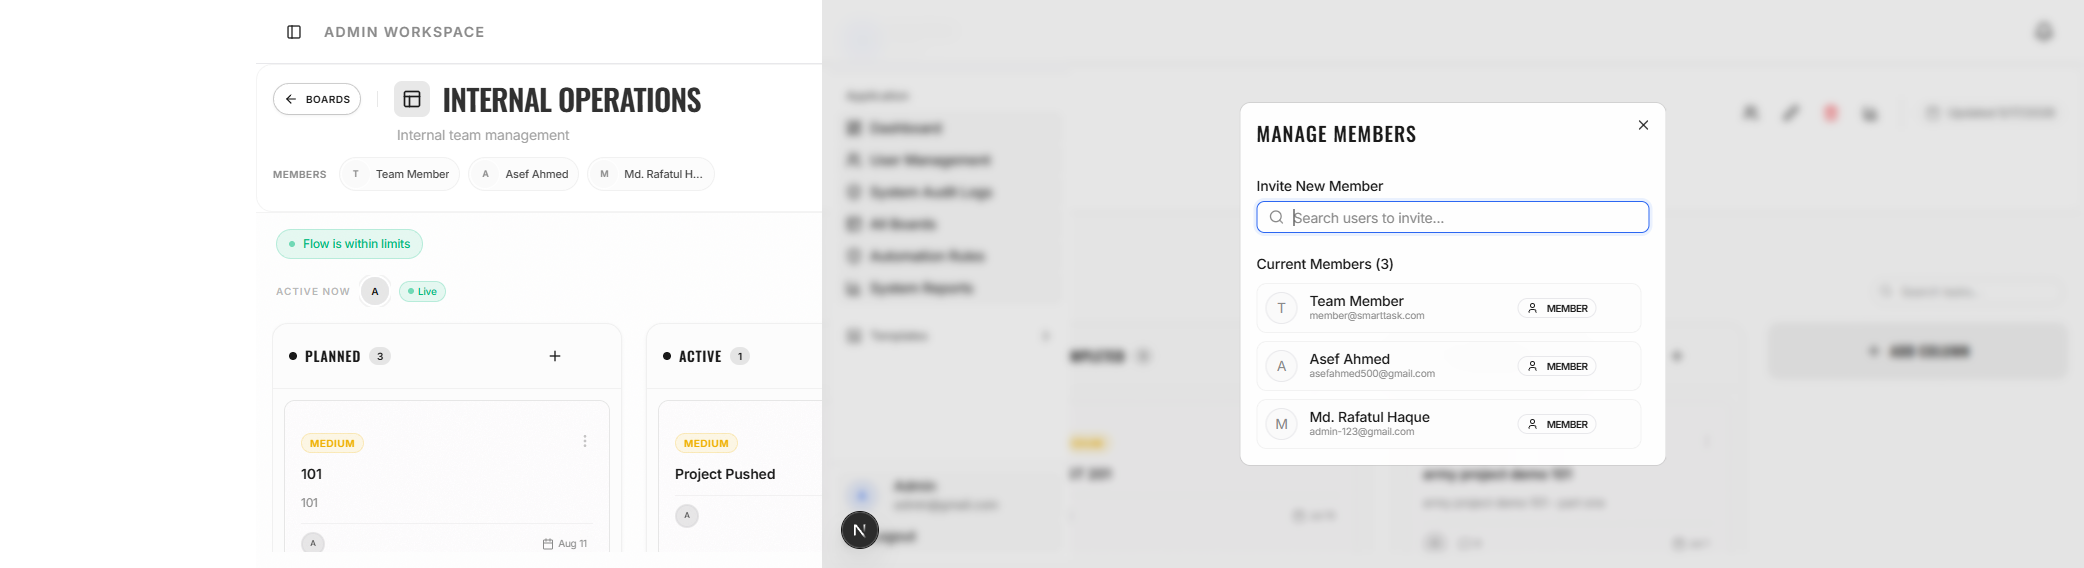
\includegraphics[width=0.9\textwidth]{figures/screenshot-board-members}
  \caption{Manage members dialog for searching and inviting users to a board.}
\end{figure}

\begin{figure}[h]
  \centering
  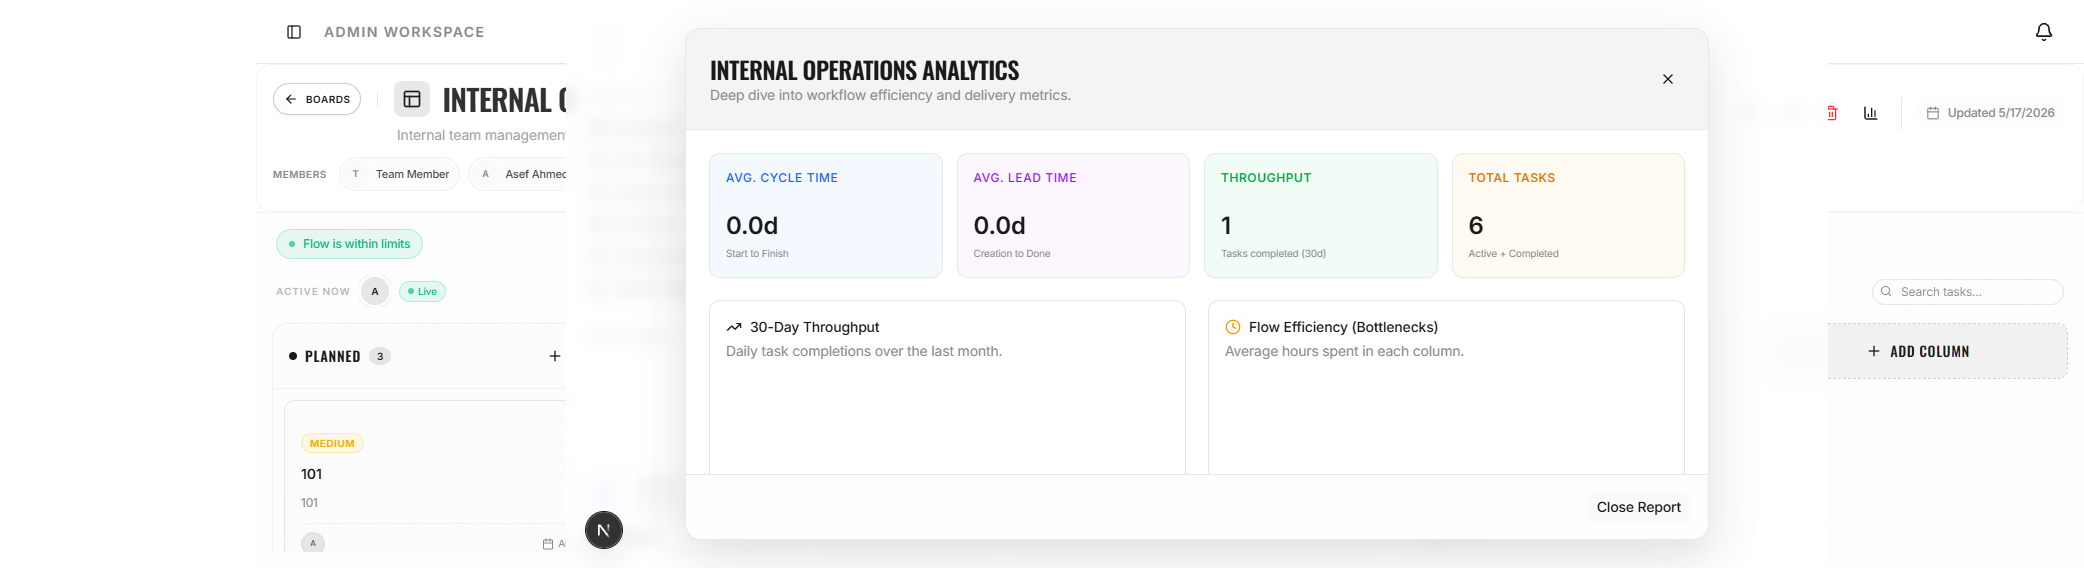
\includegraphics[width=0.9\textwidth]{figures/screenshot-board-analytics}
  \caption{Board analytics dialog with flow and throughput charts.}
\end{figure}

\subsection{Sprint and Epic Modules}
\begin{figure}[h]
  \centering
  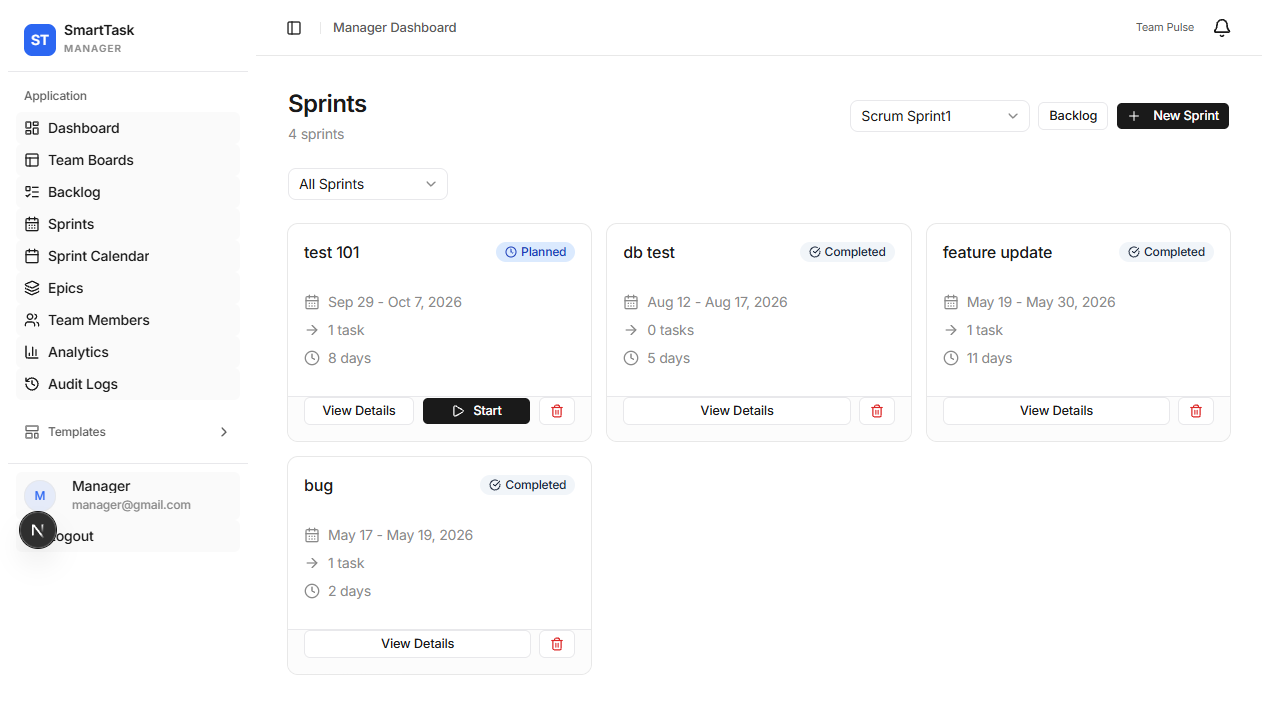
\includegraphics[width=0.9\textwidth]{figures/screenshot-sprint-list}
  \caption{Sprint list showing planned, active, and completed sprints with the
  active sprint highlighted.}
\end{figure}

\begin{figure}[h]
  \centering
  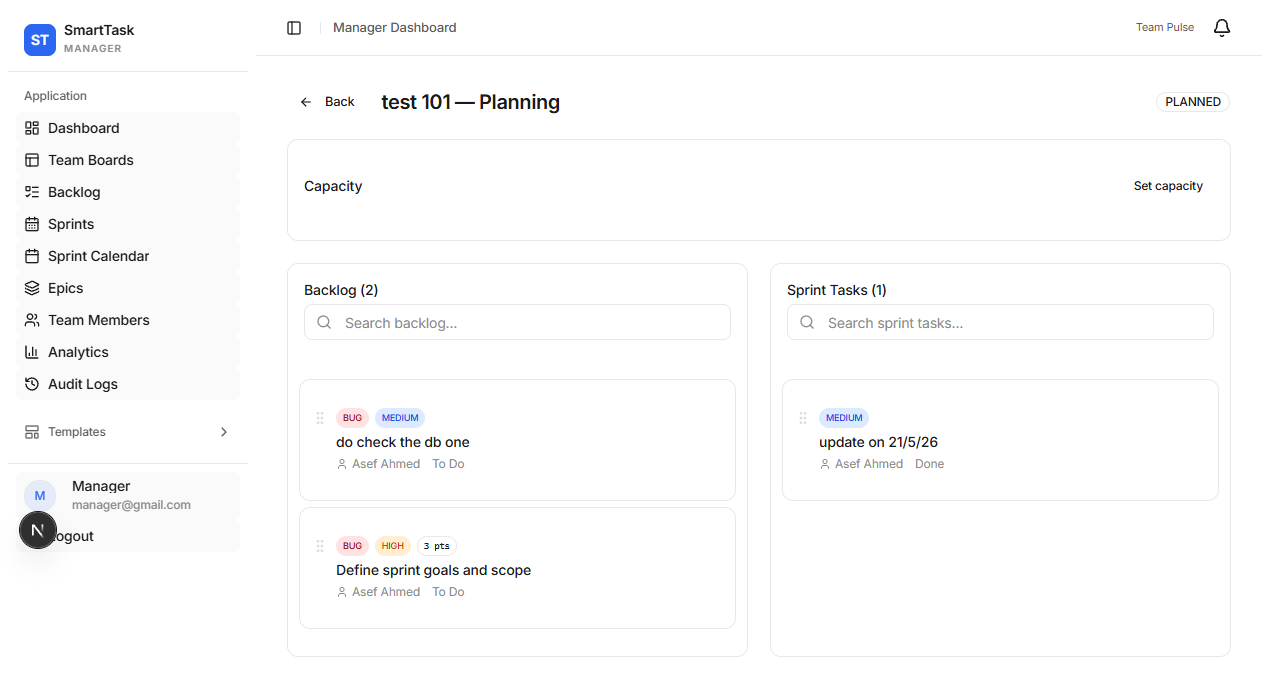
\includegraphics[width=0.9\textwidth]{figures/screenshot-sprint-planning}
  \caption{Sprint planning board with a two-panel layout for assigning backlog
  tasks to a sprint.}
\end{figure}

\begin{figure}[h]
  \centering
  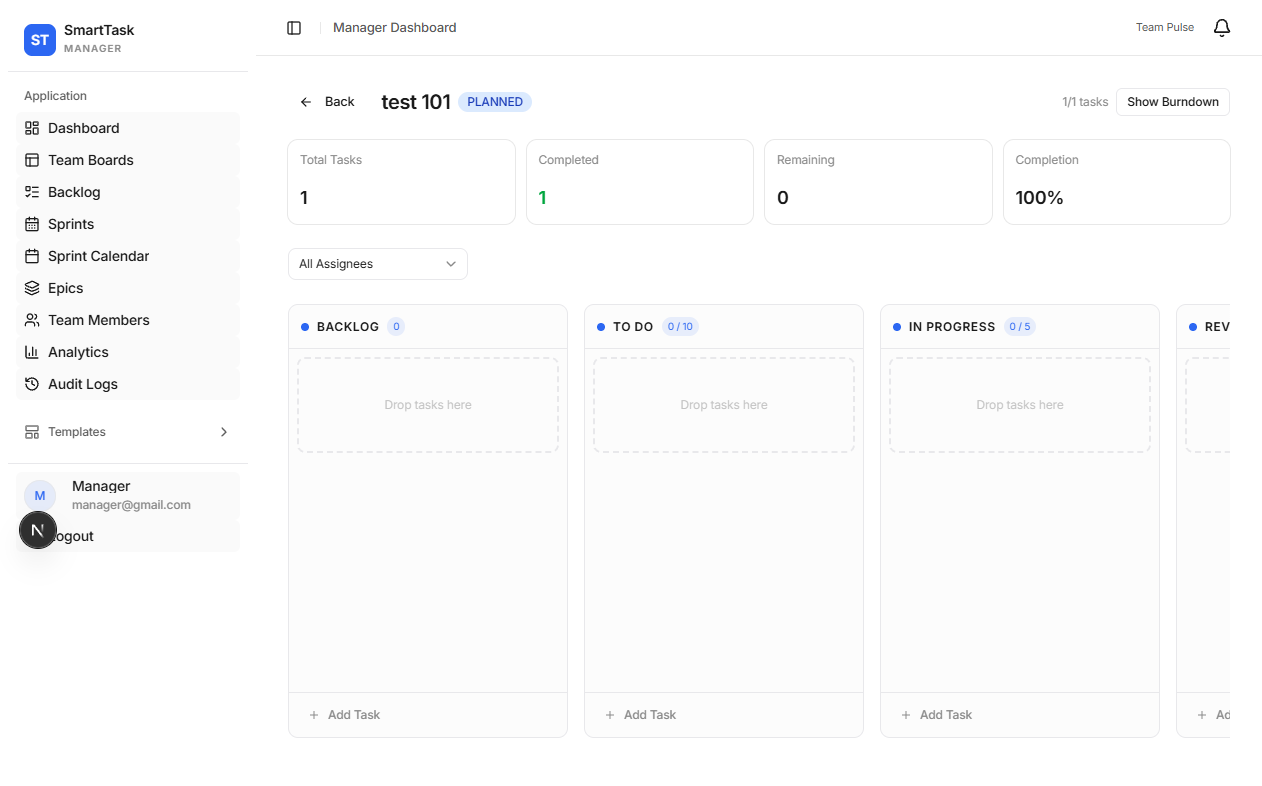
\includegraphics[width=0.9\textwidth]{figures/screenshot-sprint-board}
  \caption{Sprint-filtered Kanban board with drag-and-drop support.}
\end{figure}

\begin{figure}[h]
  \centering
  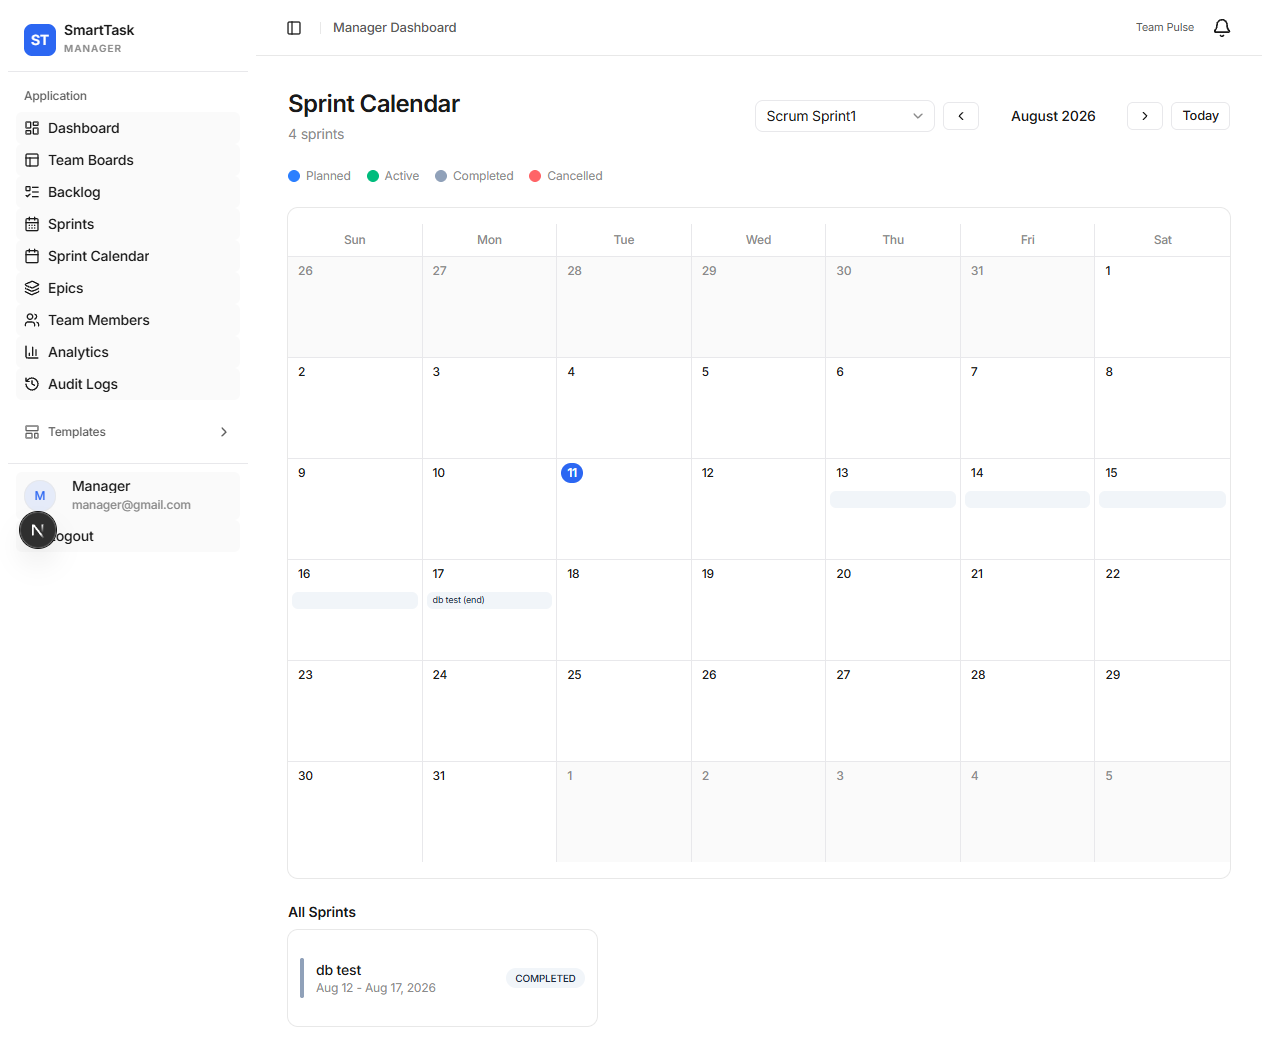
\includegraphics[width=0.9\textwidth]{figures/screenshot-sprint-calendar}
  \caption{Sprint calendar view displaying sprint bars by month.}
\end{figure}

\begin{figure}[h]
  \centering
  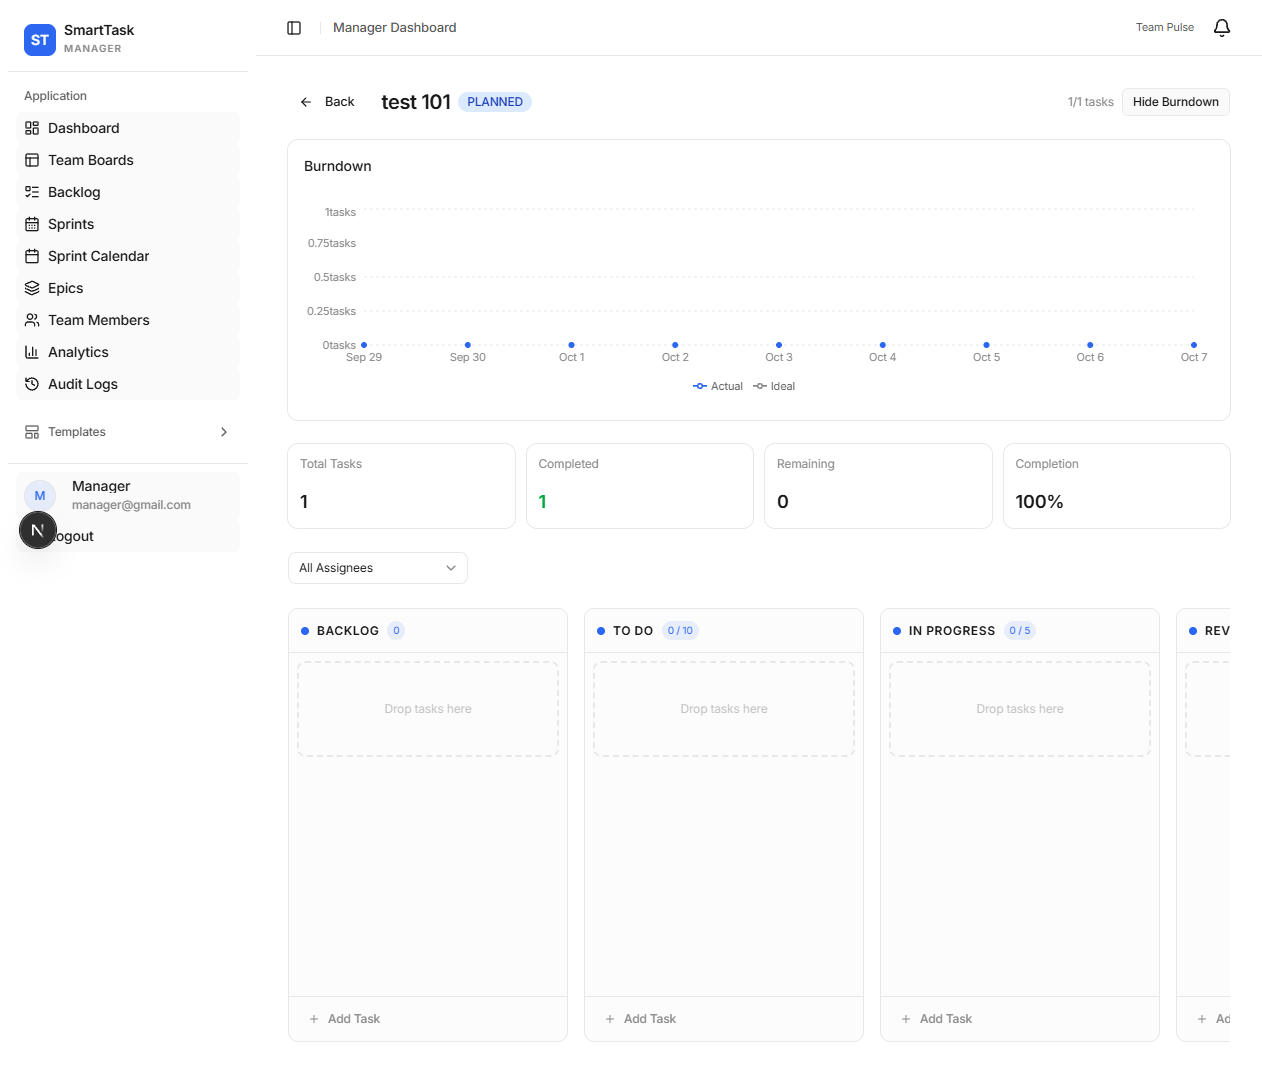
\includegraphics[width=0.9\textwidth]{figures/screenshot-sprint-burndown}
  \caption{Sprint burndown chart comparing ideal and actual completion.}
\end{figure}

\begin{figure}[h]
  \centering
  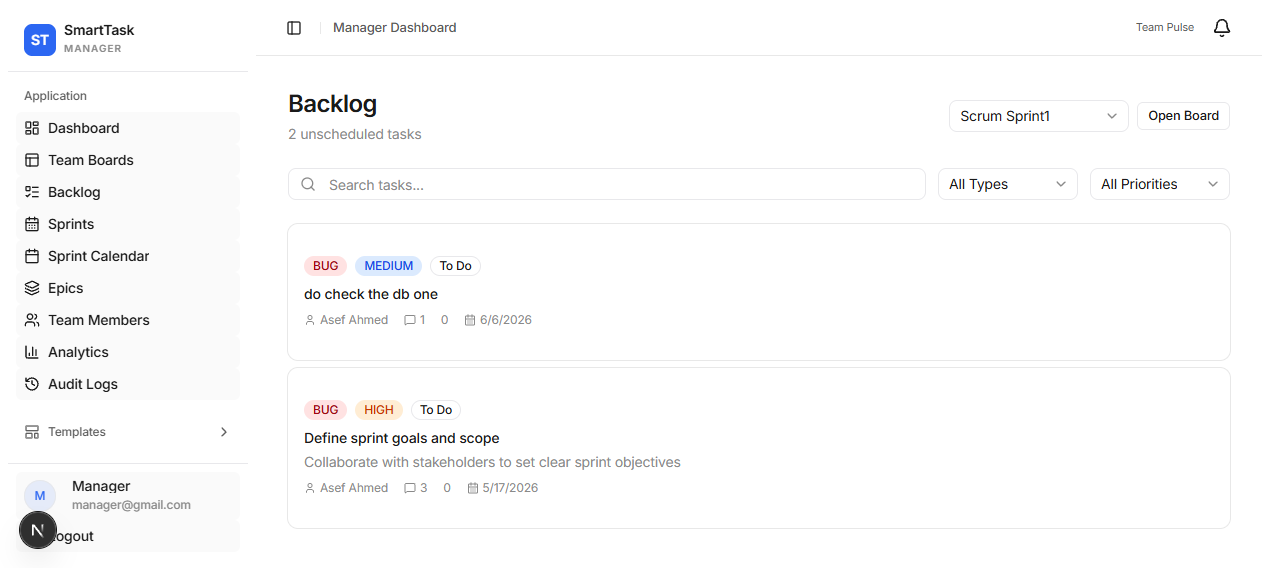
\includegraphics[width=0.9\textwidth]{figures/screenshot-backlog}
  \caption{Backlog view listing unscheduled tasks available for sprint planning.}
\end{figure}

\begin{figure}[h]
  \centering
  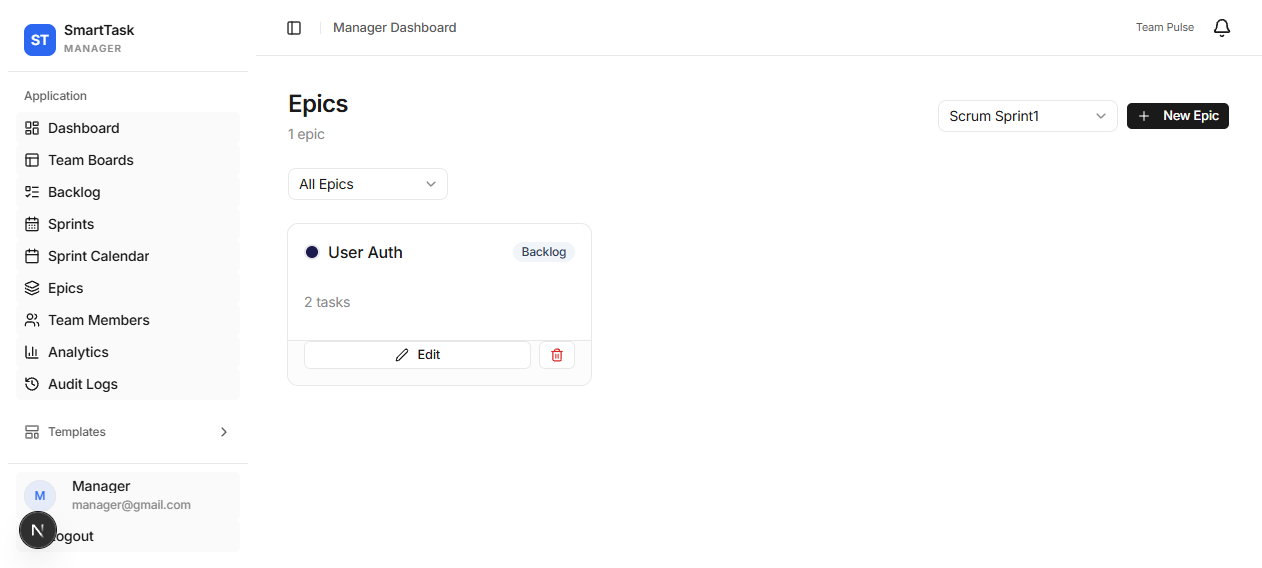
\includegraphics[width=0.9\textwidth]{figures/screenshot-epic-list}
  \caption{Epic list with progress indicators.}
\end{figure}

\subsection{Administration and Analytics Modules}
\begin{figure}[h]
  \centering
  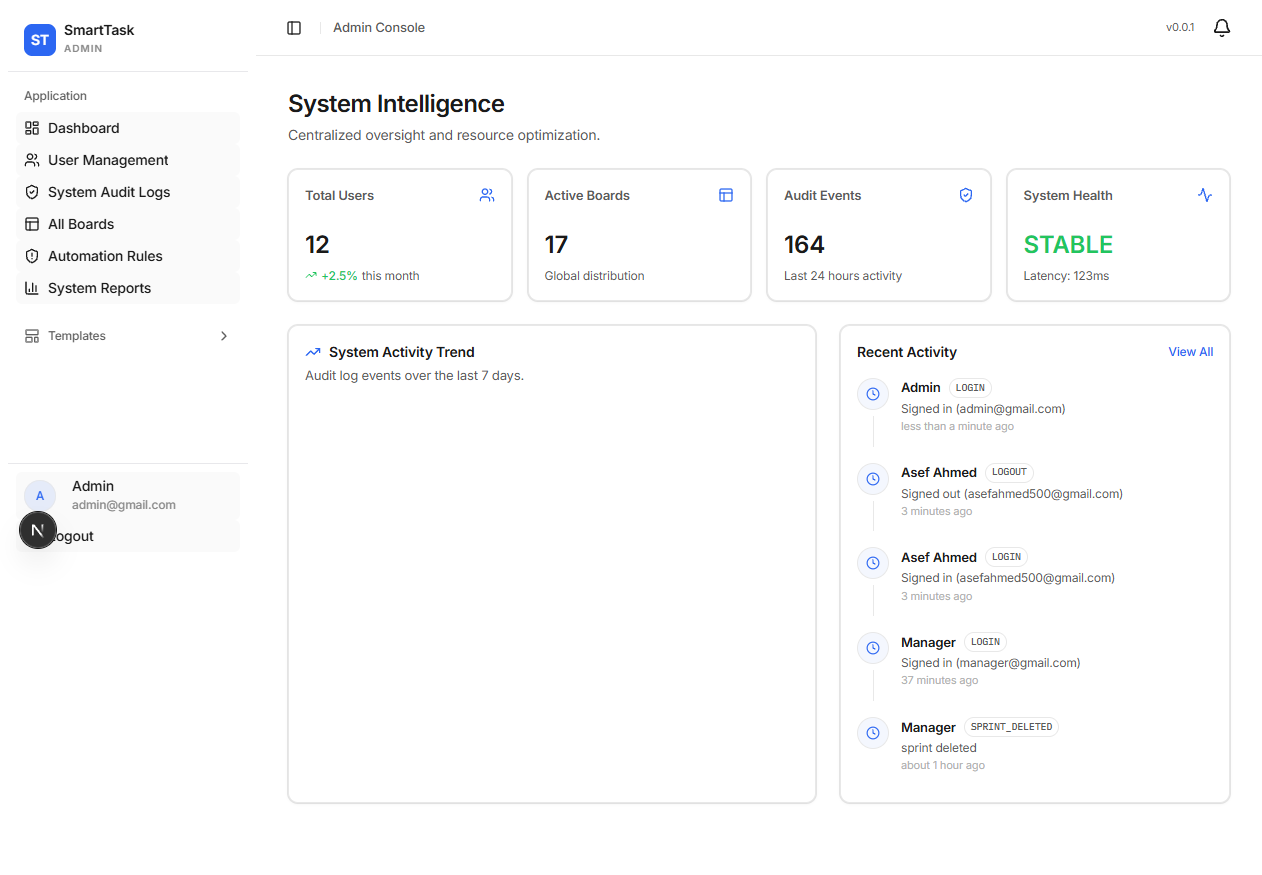
\includegraphics[width=0.9\textwidth]{figures/screenshot-admin-dashboard}
  \caption{Administrator dashboard with system statistics and activity chart.}
\end{figure}

\begin{figure}[h]
  \centering
  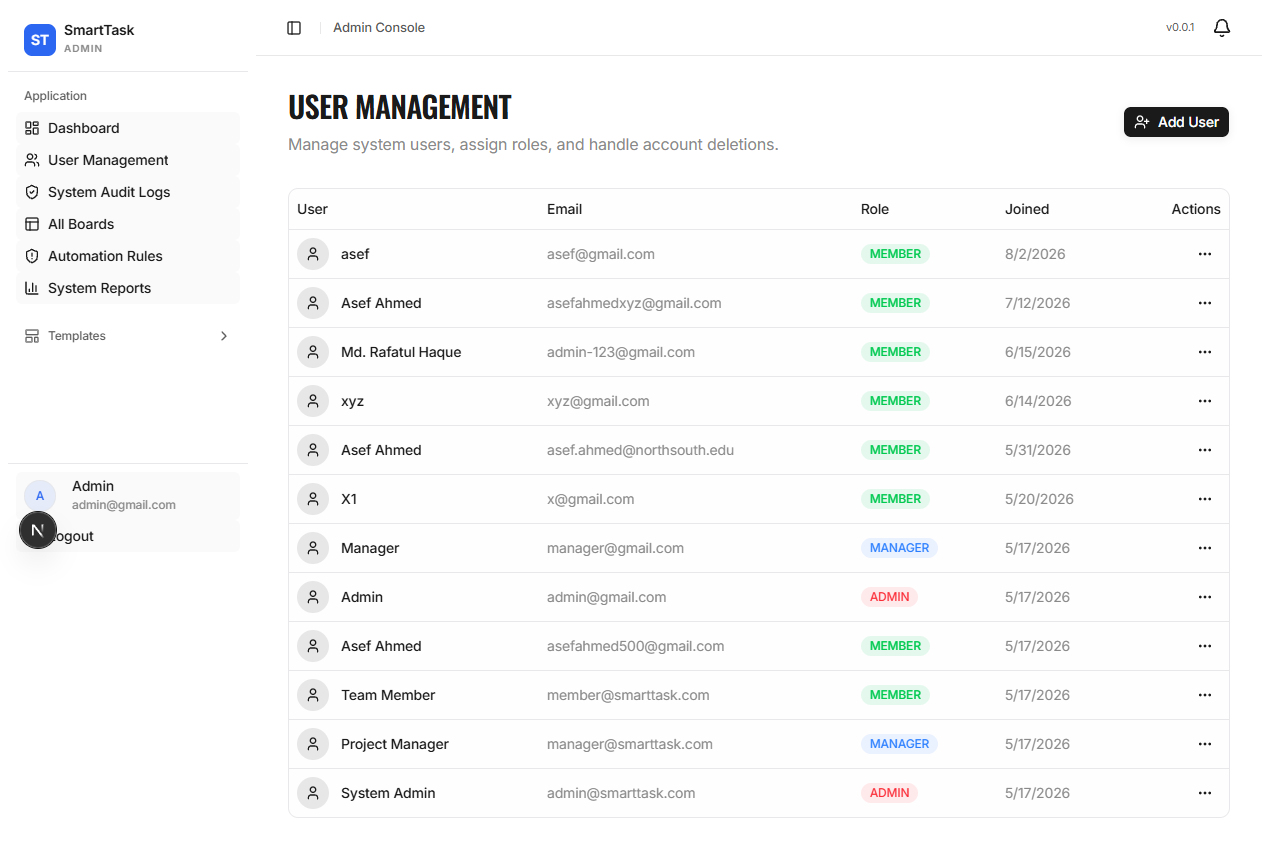
\includegraphics[width=0.9\textwidth]{figures/screenshot-admin-users}
  \caption{User management page for creating users, changing roles, and managing
  accounts.}
\end{figure}

\begin{figure}[h]
  \centering
  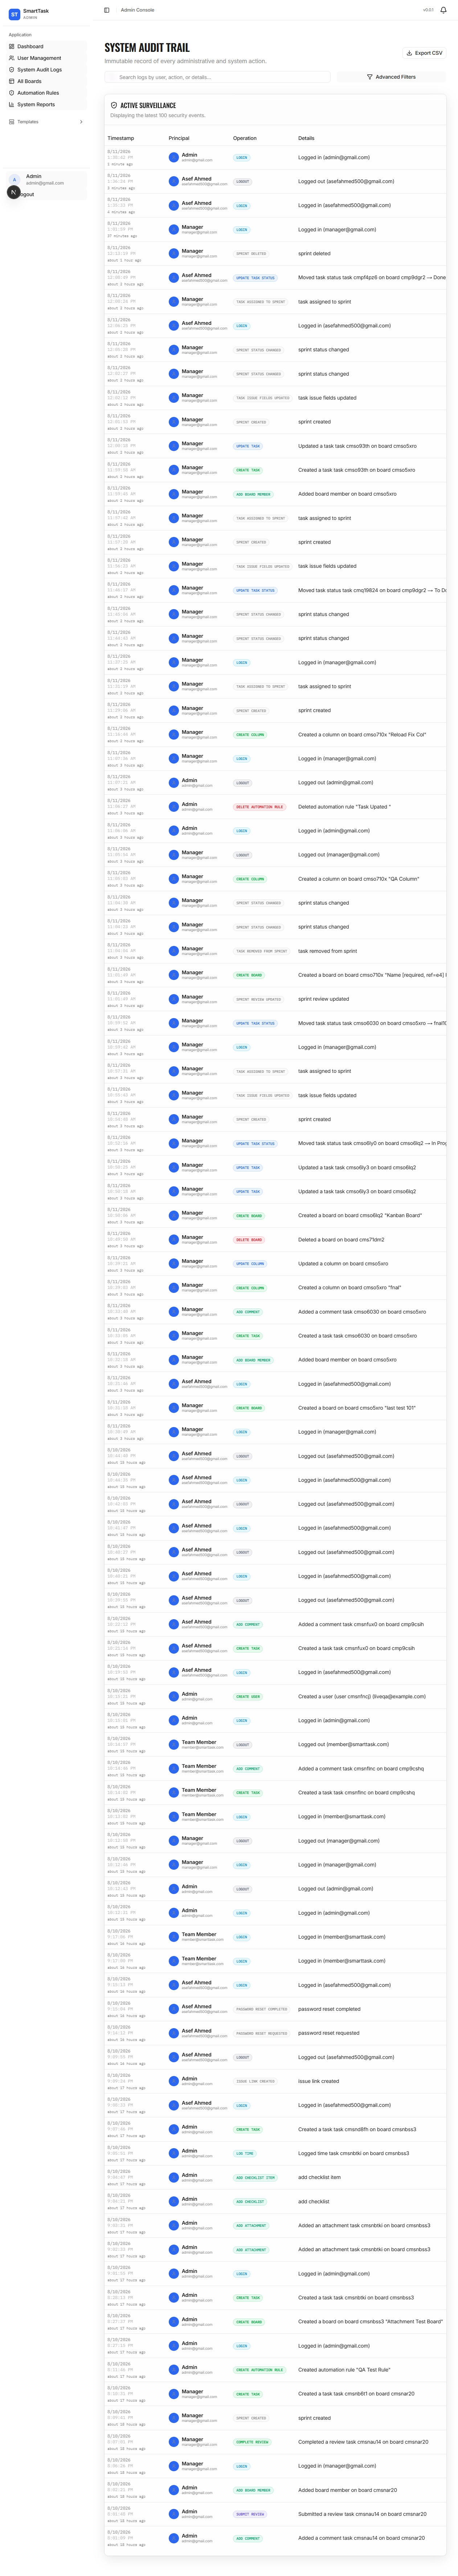
\includegraphics[width=0.9\textwidth]{figures/screenshot-admin-audit}
  \caption{System audit log viewer with filters and CSV export.}
\end{figure}

\begin{figure}[h]
  \centering
  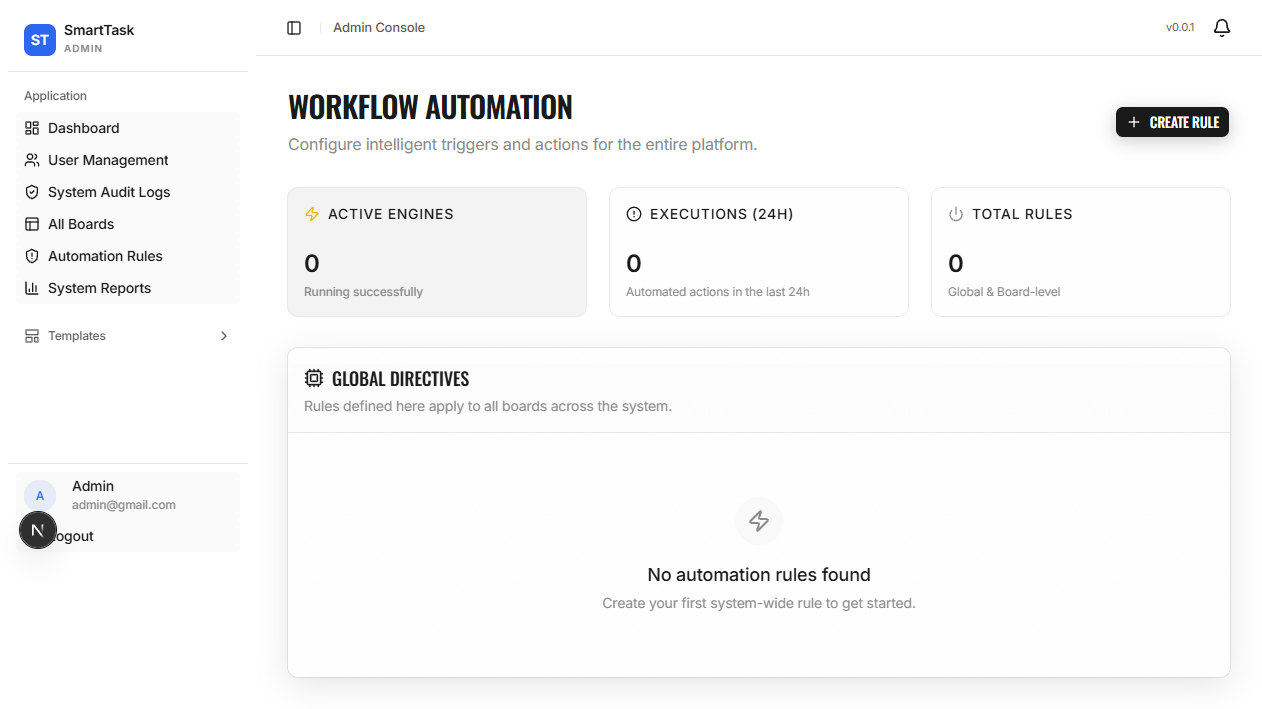
\includegraphics[width=0.9\textwidth]{figures/screenshot-admin-automation}
  \caption{Automation rules page with active engines and execution statistics.}
\end{figure}

\begin{figure}[h]
  \centering
  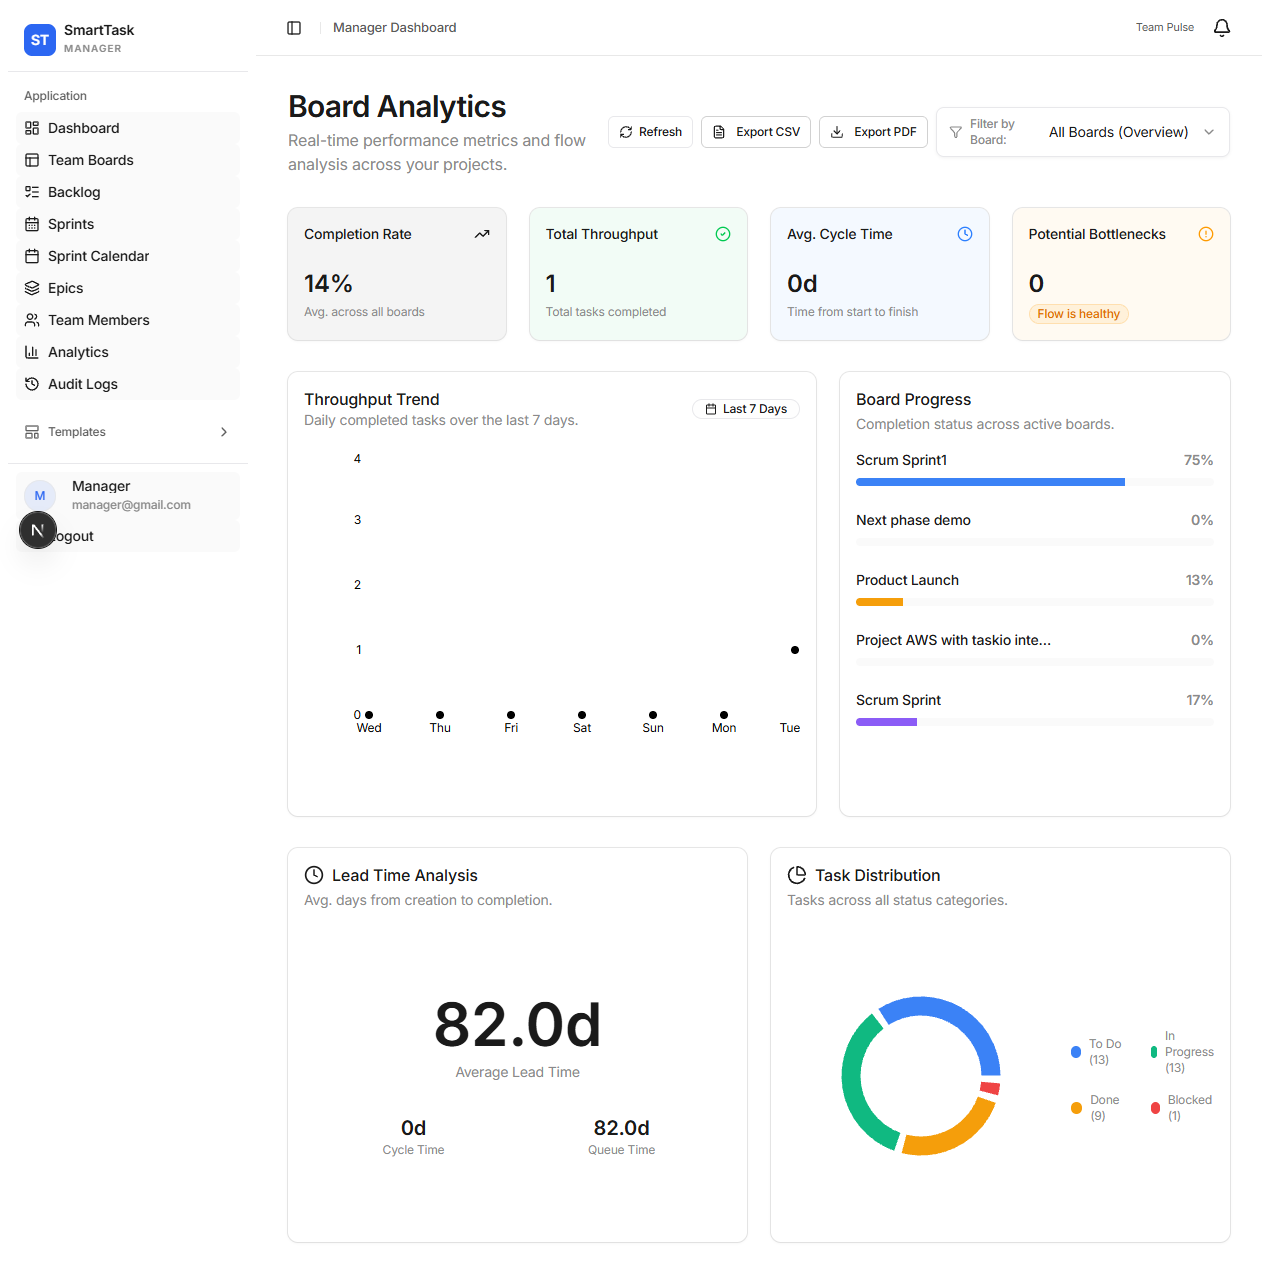
\includegraphics[width=0.9\textwidth]{figures/screenshot-manager-analytics}
  \caption{Manager analytics with throughput, cycle time, and status
  distribution charts.}
\end{figure}

\begin{figure}[h]
  \centering
  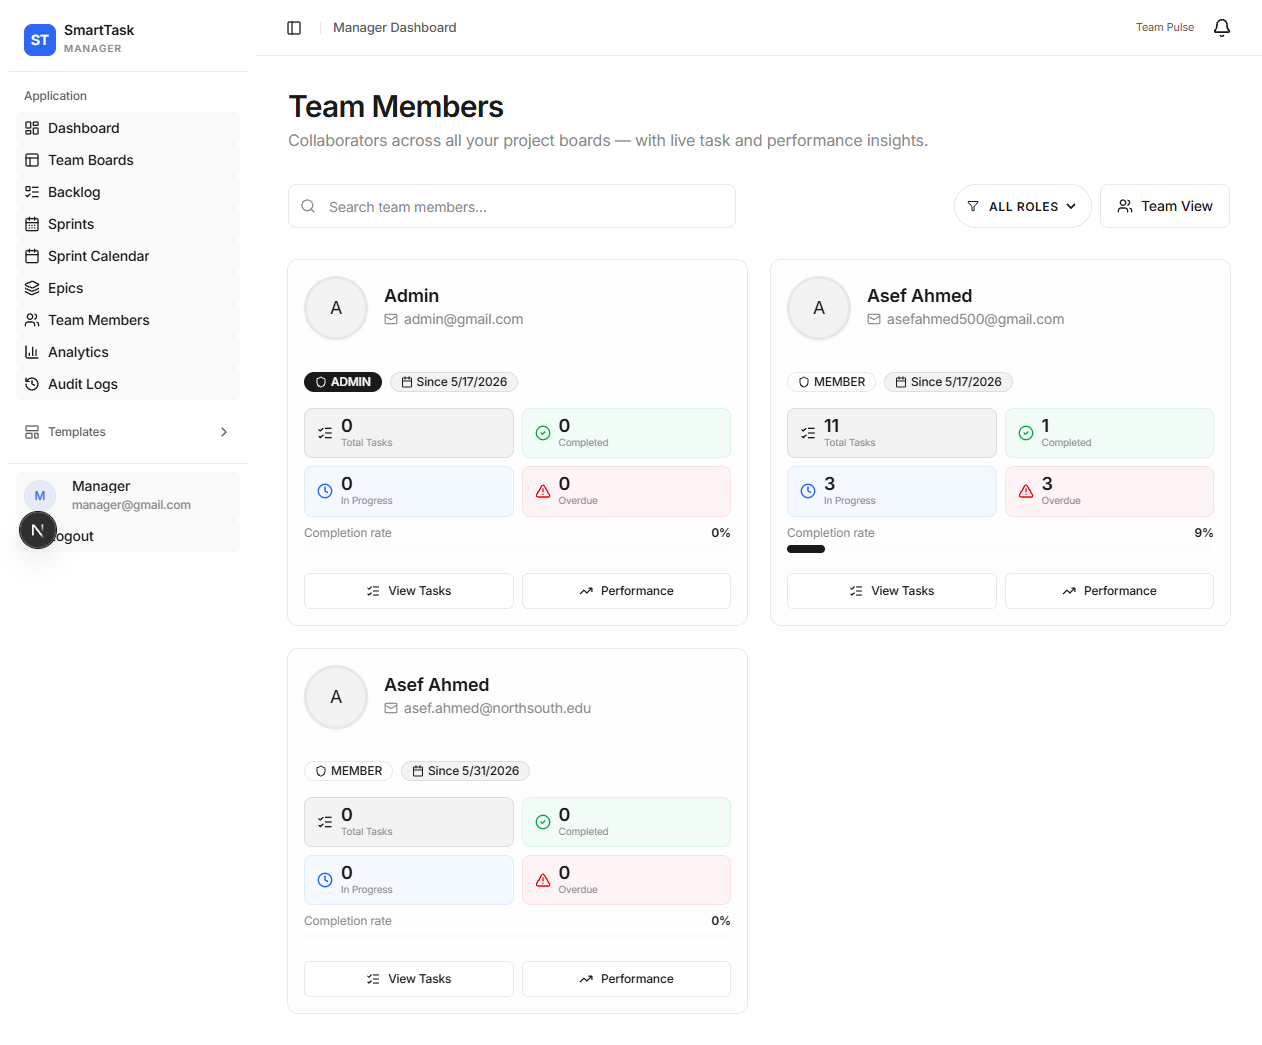
\includegraphics[width=0.9\textwidth]{figures/screenshot-manager-team}
  \caption{Team members page listing members across the manager's boards.}
\end{figure}

\begin{figure}[h]
  \centering
  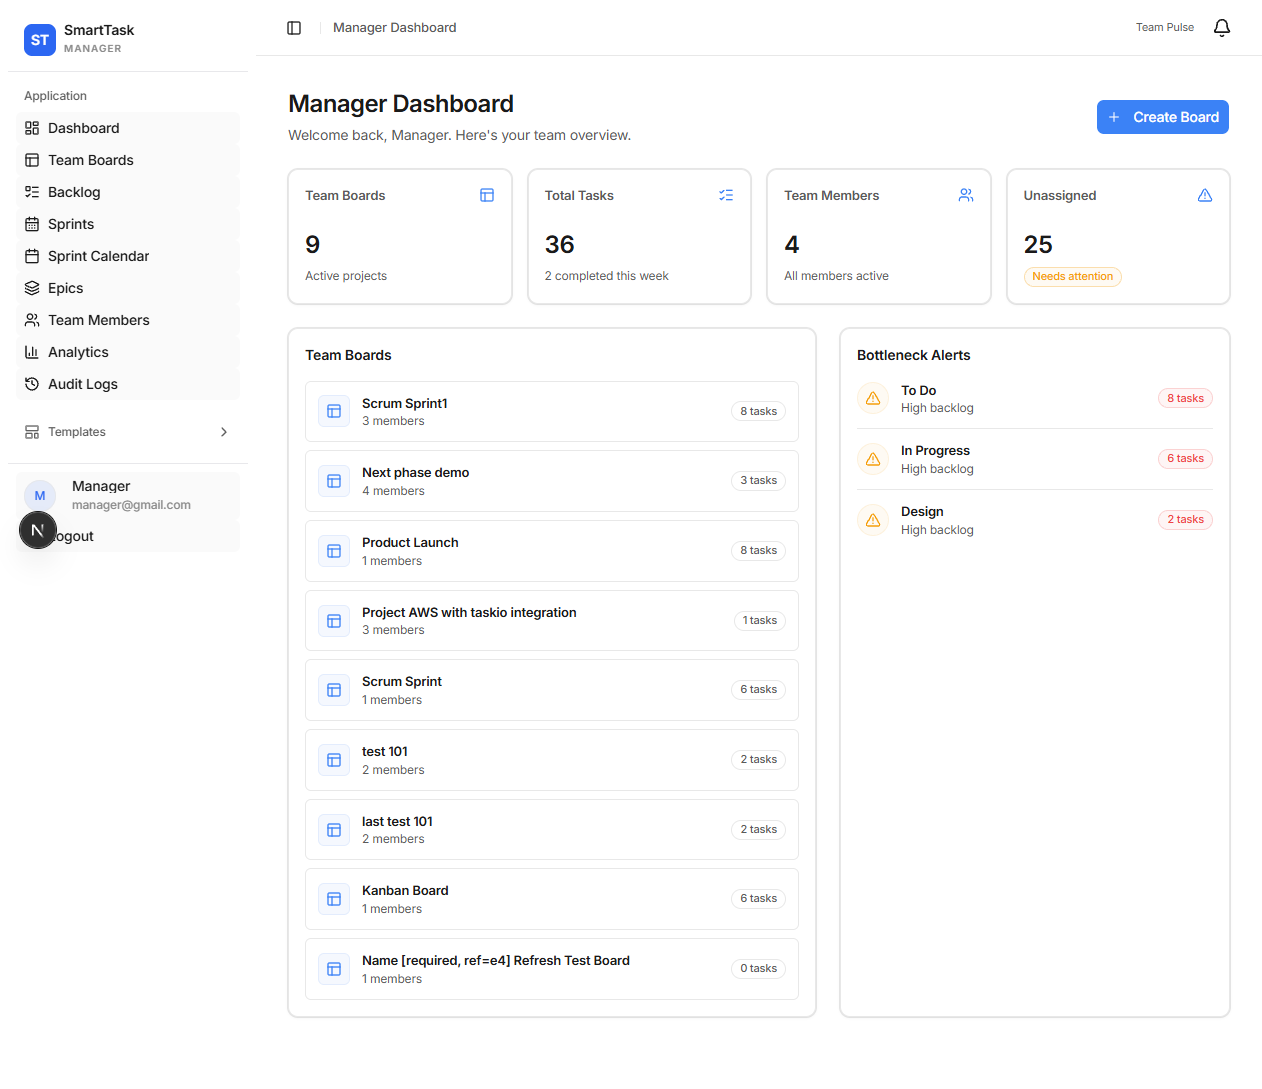
\includegraphics[width=0.9\textwidth]{figures/screenshot-notifications}
  \caption{Notification bell and notification list.}
\end{figure}

\begin{figure}[h]
  \centering
  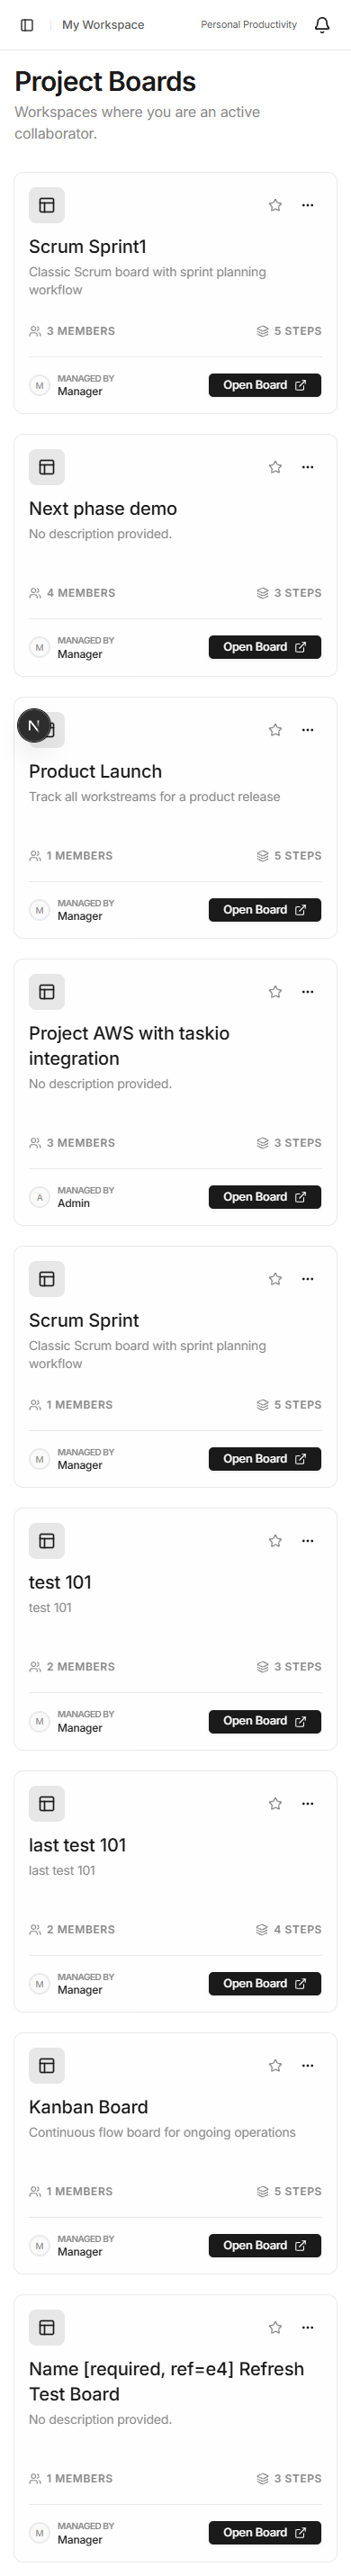
\includegraphics[width=0.9\textwidth]{figures/screenshot-mobile}
  \caption{Mobile viewport of the application showing the responsive sidebar and
  board layout.}
\end{figure}

\section{Deployment}
The application is deployed to production at
\url{https://smarttaskio.vercel.app}. The Next.js application runs on Vercel,
while the standalone Socket.IO server runs on Render, and a shared Supabase
PostgreSQL database serves both. The deployment is configured so that the
\emph{SOCKET\_INTERNAL\_TOKEN} environment variable is identical on both hosts,
allowing server actions to emit real-time notifications to any user. Deployment
is triggered through the Vercel CLI and continuous integration from the Git
repository.

\section{Database Schema}
The database is defined in a single Prisma schema and consists of the following
models: \texttt{User}, \texttt{Board}, \texttt{Column}, \texttt{Task},
\texttt{Comment}, \texttt{Reaction}, \texttt{Attachment}, \texttt{FileBlob},
\texttt{Checklist}, \texttt{ChecklistItem}, \texttt{TimeEntry}, \texttt{Review},
\texttt{Tag}, \texttt{Sprint}, \texttt{Epic}, \texttt{IssueLink},
\texttt{Notification}, \texttt{NotificationPreference}, \texttt{AutomationRule},
\texttt{AuditLog}, and \texttt{PasswordResetToken}. Critical relationships are
cascading: deleting a board removes its columns and tasks; deleting an attachment
removes its stored file blob; and deleting a task removes its comments,
checklists, time entries, and reviews.

\begin{center}
\begin{tabular}{|l|p{9.5cm}|}
\hline
\textbf{Table} & \textbf{Purpose} \\
\hline
User & Account credentials, role, active status, password version. \\
\hline
Board & Project board with owner and member relations. \\
\hline
Column & Board column with name, order, and WIP limit. \\
\hline
Task & Core work item with title, description, priority, assignee, dates, and
issue fields. \\
\hline
Comment & User comment on a task, with mention-aware content. \\
\hline
Reaction & Emoji reaction on a comment. \\
\hline
Attachment & Attachment metadata pointing to a stored file blob. \\
\hline
FileBlob & Base64-encoded file bytes backing an attachment. \\
\hline
Checklist, ChecklistItem & Checklist structure and its items with completion
state. \\
\hline
TimeEntry & Logged time against a task. \\
\hline
Review & Review request with status and feedback. \\
\hline
Tag & Board-scoped or global labels. \\
\hline
Sprint, Epic & Agile planning entities associated with a board. \\
\hline
IssueLink & Directed relations between tasks. \\
\hline
Notification, NotificationPreference & Notification records and per-user
delivery preferences. \\
\hline
AutomationRule & Trigger/action rules for workflow automation. \\
\hline
AuditLog & Immutable log of user actions. \\
\hline
PasswordResetToken & One-hour tokens for password recovery. \\
\hline
\end{tabular}
\end{center}

\section{Key Implementation Decisions}
\subsection{Authentication}
A JWT is created at login and stored in an HTTP-only, SameSite=Lax cookie. The
\emph{getSession} helper re-validates the user's active status and password
version on every call, so password changes immediately invalidate existing
sessions. Socket.IO connections authenticate by fetching the session token from a
same-origin API route; the token is held in memory and never written to
localStorage, eliminating stale-token mismatches when switching accounts.
\subsection{Real-Time Collaboration}
A standalone Socket.IO server registers each connection to a user room and to
board rooms. Server actions emit events after database commits, and the socket
server relays them only to authorised recipients. A shared internal token allows
the application server to notify any user, while browser clients may only notify
themselves.
\subsection{File Uploads}
Attachments are uploaded to a server-side route that validates size and type,
checks board permission, and stores the file bytes base64-encoded in the
\texttt{FileBlob} table. A serving route returns the bytes with the appropriate
content type and download disposition.
\subsection{Bundle Optimisation}
The Recharts library is lazy-loaded through \texttt{next/dynamic} wrappers so that
heavy charting code is fetched only when a chart is actually displayed.

% ----------------------------------------------------------------------------
% CHAPTER 6 — TESTING AND RESULTS
% ----------------------------------------------------------------------------
\chapter{Testing and Results}
\label{ch:testing}

\section{Testing Strategy}
The application was tested through static analysis (TypeScript type-checking and
production builds) and extensive interactive browser-based testing covering all
roles, all routes, and all major services. A comprehensive quality-assurance pass
executed real operations -- creating boards and tasks, adding comments, submitting
and approving reviews, creating sprints, uploading attachments, and switching
between accounts -- verifying both immediate feedback and persistence after
reload. Database state was inspected directly to confirm that operations persisted
and cascaded correctly.

\section{Unit Testing}
\begin{center}
\begin{tabular}{|l|l|p{4.2cm}|p{3cm}|p{2.6cm}|c|}
\hline
\textbf{ID} & \textbf{Module} & \textbf{Description} & \textbf{Input} & \textbf{Expected Output} & \textbf{Status} \\
\hline
UT-01 & Auth & Login with valid credentials & admin@gmail.com / admin123 & Redirect to /admin & Pass \\
\hline
UT-02 & Auth & Login with invalid password & admin@gmail.com / wrong & 401 Invalid credentials & Pass \\
\hline
UT-03 & Board & Create board & name, description & Board persisted & Pass \\
\hline
UT-04 & Column & Set WIP limit & integer 0--100 & Limit saved & Pass \\
\hline
UT-05 & Task & Create task with assignee & title, assignee & Task created + notification & Pass \\
\hline
UT-06 & Comment & Add comment & content & Comment visible & Pass \\
\hline
UT-07 & Checklist & Add checklist item & content & Item persisted & Pass \\
\hline
UT-08 & Time & Log time entry & 60 minutes & Entry persisted & Pass \\
\hline
UT-09 & Review & Submit review, self-review & self as reviewer & Blocked & Pass \\
\hline
UT-10 & User & Create user (admin) & valid data & User appears in list & Pass \\
\hline
\end{tabular}
\end{center}

\section{Integration Testing}
\begin{center}
\begin{tabular}{|l|p{3.5cm}|p{4.5cm}|p{4.5cm}|c|}
\hline
\textbf{ID} & \textbf{Modules} & \textbf{Description} & \textbf{Expected Output} & \textbf{Status} \\
\hline
IT-01 & Auth + Proxy & Member accesses /admin URL directly & Redirect to /member & Pass \\
\hline
IT-02 & Task + Socket & Manager creates task on shared board & Admin viewer sees it live & Pass \\
\hline
IT-03 & Review + Workflow & Manager approves review & Task auto-moves to Done column & Pass \\
\hline
IT-04 & Sprint + Backlog & Complete active sprint & Incomplete tasks return to backlog & Pass \\
\hline
IT-05 & Attachment + DB & Upload file, delete attachment & Blob cascade-deleted (no orphans) & Pass \\
\hline
IT-06 & Auth + Session & Switch account after logout & No stale JWT on socket & Pass \\
\hline
IT-07 & Automation + Task & Create automation rule, trigger event & Rule executes + logged & Pass \\
\hline
IT-08 & Audit + Undo & Perform action, view audit log & Entry recorded & Pass \\
\hline
\end{tabular}
\end{center}

\section{Performance Testing}
\begin{center}
\begin{tabular}{|l|l|p{4.5cm}|p{3.5cm}|c|}
\hline
\textbf{ID} & \textbf{Area} & \textbf{Description} & \textbf{Measured} & \textbf{Status} \\
\hline
PT-01 & Build & Production build with type-check & Success, all routes compiled & Pass \\
\hline
PT-02 & Page load & Login page load & Fast, no runtime errors & Pass \\
\hline
PT-03 & Board render & Kanban board with tasks & Renders without errors & Pass \\
\hline
PT-04 & Lazy charts & Recharts loaded on demand & Chart fetched only when shown & Pass \\
\hline
PT-05 & Responsive & 390px viewport & No horizontal overflow & Pass \\
\hline
PT-06 & Real-time & Socket event propagation & Live update within seconds & Pass \\
\hline
\end{tabular}
\end{center}

\section{Testing Results Summary}
All unit, integration, and performance test cases recorded above passed. The
interactive browser-based quality assurance pass verified authentication across
all three roles, board and task creation with persistence, comments, reviews with
automatic workflow transitions, sprint creation, attachment upload and serving,
issue linking, checklist and time tracking, role-based access restrictions, mobile
responsiveness, and real-time collaboration. All test data was removed after
testing, leaving the production database in its baseline state.

% ----------------------------------------------------------------------------
% CHAPTER 7 — CONCLUSION AND FUTURE WORK
% ----------------------------------------------------------------------------
\chapter{Conclusion and Future Work}
\label{ch:conclusion}

\section{Conclusion}
This project successfully designed and implemented SmartTask, a real-time
collaborative Kanban-based task management system. The application delivers a
complete role-based workflow covering boards, tasks, sprints, epics, reviews,
automation, notifications, and auditing, secured with HTTP-only-cookie
authentication and guarded at both the middleware and server-action layers. A
standalone Socket.IO server provides real-time board updates and notifications,
and a database-backed file upload mechanism replaces client-side file handling.
The system was validated through extensive interactive testing across all roles
and services, and it is deployed and running in production. The project
demonstrates a cohesive integration of modern web technologies to solve a real
collaboration problem.

\section{Limitations}
The following limitations were identified during the project:
\begin{itemize}
  \item Drag-and-drop interaction could not be fully automated in headless
        browser testing; its underlying status-change logic was nevertheless
        verified through alternative workflows.
  \item Offline mode queues mutations for later synchronisation, but the full
        queue-and-reconcile scenario was not exhaustively exercised in automated
        tests.
  \item File storage is database-backed base64, which is simple and
        serverless-friendly but consumes database storage for large files.
  \item The undo mechanism operates within a short 30-second window and does not
        support redo.
  \item Real-time testing was performed on a local development cluster and a
        single production deployment; very large concurrent user loads were not
        benchmarked.
\end{itemize}

\section{Future Work}
Plausible directions for future development include:
\begin{itemize}
  \item Replacing database-backed file storage with object storage (for example,
        S3 or R2) and signed URLs.
  \item Adding a full offline-first experience with conflict resolution and a
        durable operation queue.
  \item Introducing multi-board team workspaces with nested team hierarchies and
        fine-grained custom roles.
  \item Adding a REST/GraphQL public API to support third-party integrations.
  \item Implementing a redo capability alongside the existing undo mechanism, and
        richer reporting with exportable charts.
\end{itemize}

% ----------------------------------------------------------------------------
% REFERENCES
% ----------------------------------------------------------------------------
\begin{thebibliography}{9}
\bibitem{trello} Trello. \emph{Trello: Manage Your Team's Projects From Anywhere.}
Available at: \url{https://trello.com} (Accessed: 10 August 2026).
\bibitem{jira} Atlassian. \emph{Jira Software: The #1 Software Development Tool.}
Available at: \url{https://www.atlassian.com/software/jira} (Accessed: 10 August 2026).
\bibitem{asana} Asana. \emph{Asana: Work Management Platform.}
Available at: \url{https://asana.com} (Accessed: 10 August 2026).
\bibitem{kanban} D.~J. Anderson. \emph{Kanban: Successful Evolutionary Change for
Your Technology Business.} Blue Hole Press, 2010.
\bibitem{nextjs} Vercel. \emph{Next.js: The React Framework.}
Available at: \url{https://nextjs.org} (Accessed: 10 August 2026).
\bibitem{prisma} Prisma. \emph{Prisma ORM Documentation.}
Available at: \url{https://www.prisma.io/docs} (Accessed: 10 August 2026).
\bibitem{socketio} Socket.IO. \emph{Socket.IO Documentation.}
Available at: \url{https://socket.io/docs} (Accessed: 10 August 2026).
\bibitem{jwt} IETF. \emph{RFC 7519: JSON Web Token (JWT).}
Available at: \url{https://datatracker.ietf.org/doc/html/rfc7519} (Accessed: 10 August 2026).
\bibitem{supabase} Supabase. \emph{Supabase: The Open Source Firebase Alternative.}
Available at: \url{https://supabase.com} (Accessed: 10 August 2026).
\end{thebibliography}
